\documentclass[xcolor=dvipsnames]{beamer}
%\documentclass{beamer}

%\documentclass[handout]{beamer}

%\usepackage[table]{xcolor}
\mode<presentation> {
  \usetheme{Boadilla}
%  \usetheme{Pittsburgh}
%\usefonttheme[2]{sans}
\renewcommand{\familydefault}{cmss}
%\usepackage{lmodern}
%\usepackage[T1]{fontenc}
%\usepackage{palatino}
%\usepackage{cmbright}
  \setbeamercovered{transparent}
\useinnertheme{rectangles}
}
\usepackage{soul}
\setbeamercolor{normal text}{fg=black}
\setbeamercolor{structure}{fg= black}
\beamertemplatesolidbackgroundcolor{white}  \setbeamercolor{alerted
text}{fg=red}
\usepackage{amsmath}
\usepackage[english]{babel}
\usepackage[latin1]{inputenc}
\usepackage{times}
\usepackage[T1]{fontenc}
\usepackage{colortbl}
\usepackage{framed}
\setbeamercovered{invisible} %% <--- I ADDED THIS
\usepackage{color}
\definecolor{gold}{rgb}{0.85,0.66,0}
\usepackage{cancel}
\usepackage{comment}
\usepackage{enumerate}
\usepackage{multirow}
\usepackage{fancybox}

% === check mark
\usepackage{pifont}
\newcommand{\cmark}{\ding{51}}
\newcommand{\xmark}{\ding{55}}

% === tikz for pictures ===
\usepackage{tikz}
\usepackage[latin1]{inputenc}
\usetikzlibrary{shapes,arrows,trees,fit,positioning}
\usepackage{booktabs} % To thicken table lines

% ==== dotted lines in tables ===
\usepackage{arydshln}
\usepackage[normalem]{ulem}

% === dcolumn package ===
\usepackage{dcolumn}
\newcolumntype{.}{D{.}{.}{-1}}
\newcolumntype{d}[1]{D{.}{.}{#1}}

% === new commands ===
\newcommand\ud{\mathrm{d}}
\newcommand\dist{\buildrel\rm d\over\sim}
\newcommand\ind{\stackrel{\rm indep.}{\sim}}
\newcommand\iid{\stackrel{\rm i.i.d.}{\sim}}
\newcommand\logit{{\rm logit}}
\renewcommand\r{\right}
\renewcommand\l{\left}
\newcommand\Var{{\rm Var}}
\newcommand\var{{\rm var}}
\newcommand\Cov{{\rm Cov}}
\newcommand\bone{\mathbf{1}}
\newcommand\E{\mathbb{E}}
\newcommand\wX{\widetilde{X}}
\newcommand\wT{\widetilde{T}}
\newcommand\independent{\protect\mathpalette{\protect\independenT}{\perp}}
\def\independenT#1#2{\mathrel{\rlap{$#1#2$}\mkern2mu{#1#2}}}


 \newenvironment{changemargin}[3]{%
 \begin{list}{}{%
 \setlength{\topsep}{0pt}%
 \setlength{\leftmargin}{#1}%
 \setlength{\rightmargin}{#2}%
 \setlength{\topmargin}{#3}%
 \setlength{\listparindent}{\parindent}%
 \setlength{\itemindent}{\parindent}%
 \setlength{\parsep}{\parskip}%
 }%
 \item[]}{\end{list}}


\newcommand\bX{\mathbf{X}}
\newcommand\bB{\mathbf{B}}
\newcommand\bD{\mathbf{D}}
\newcommand\bM{\mathbf{M}}
\newcommand\bH{\mathbf{H}}
\newcommand\bI{\mathbf{I}}
\newcommand\bG{\mathbf{G}}
\newcommand\bR{\mathbf{R}}
\newcommand\bS{\mathbf{S}}
\newcommand\bV{\mathbf{V}}
\newcommand\bW{\mathbf{W}}
\newcommand{\argmin}{\operatornamewithlimits{argmin}}
\newcommand{\argmax}{\operatornamewithlimits{argmax}}
\newcommand{\indep}{\mbox{$\perp\!\!\!\perp$}}
\def\independenT#1#2{\mathrel{\rlap{$#1#2$}\mkern2mu{#1#2}}}
\DeclareMathOperator{\sgn}{sgn}
\newcommand\spacingset[1]{\renewcommand{\baselinestretch}%
{#1}\small\normalsize}
\newcommand\ex{\colorbox{princetonorange}{\color{princetonblack}\textsc{Example}} }
\definecolor{princetonorange}{RGB}{245, 128, 37}
\definecolor{princetonblack}{RGB}{0,0,0}

% == theorems
\setbeamertemplate{theorems}[numbered]
\newcounter{asm}
\setcounter{asm}{0}
\newtheorem{assumption}[asm]{Assumption}
\newtheorem{prop}{Proposition}

% === if you want more than one slides on one page ===
\usepackage{pgfpages}
%\setbeameroption{show notes on second screen}
%\pgfpagesuselayout{2 on 1}[letterpaper,border shrink = 5mm]

%%%%%%%%%%%%%%%%%%%%%%%%%%%%%%%%%%%%%%%%%%%%%%%%%%%%%%%%%%%%%%%%%%%%%%

% If you wish to uncover everything in a step-wise fashion, uncomment
% the following command:
%\beamerdefaultoverlayspecification{<+->}


\title[Shifting Priorities and Capacity]{\Large The Effects of Shifting Prioirites and Capacity on Policy Work and Constituency Service: Evidence from a Census of Legislator Requests to U.S. Federal Agencies}
\author[Powell]{\large Eleanor Neff Powell}
\institute[Wisconsin]{\normalsize University of Wisconsin-Madison\\
{\small Joint work with Devin Judge-Lord and Justin Grimmer}}
%\author[Grimmer]{\large Justin Grimmer}
%\institute[Stanford]{\normalsize Stanford University\\
%{\small Joint work with Devin Judge-Lord and Eleanor Neff Powell}}
%\date{}

\begin{document}

\frame{\titlepage}

%%%%%%%%%%%%%%%%%%%%%%%%%%%%
\begin{frame}
\frametitle{Legislative Effort and Experience in Washington}

\Large 

\begin{itemize}
\item[-] How do legislators' attention and effort change with power and experience?
\bigskip

\item[-] Do constituents face a trade off between influence in Washington and constituency service at home?
\end{itemize} 
\end{frame}
%%%%%%%%%%%%%%%%%%%%%%%%%%%
\begin{frame}


\scalebox{0.5}{\includegraphics{../figs/SteyerPresident.jpg}}

``There's a widespread perception that the longer an elected official serves in Congress, the less connected they are to their constituent"


\end{frame}
%%%%%%%%%%%%%%%%%%%%%%%%%%

\begin{frame}


\scalebox{0.5}{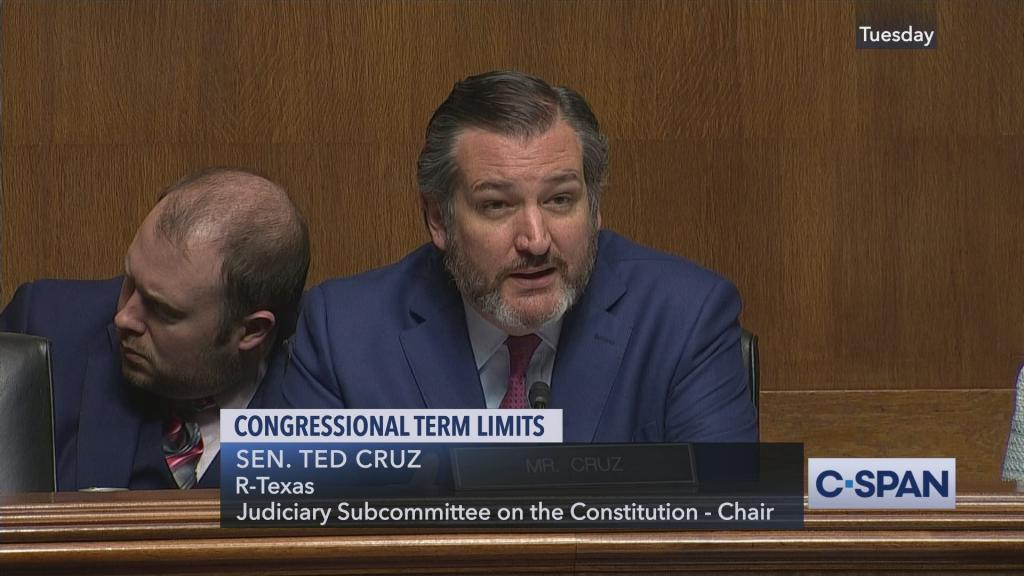
\includegraphics{../figs/CruzHearing1.jpg}}

``...members of Congress get re-elected and the system works for everyone except the American people.  This kind of self-interest builds on itself as members spend more time in office"


\end{frame}


\begin{frame}


\scalebox{0.4}{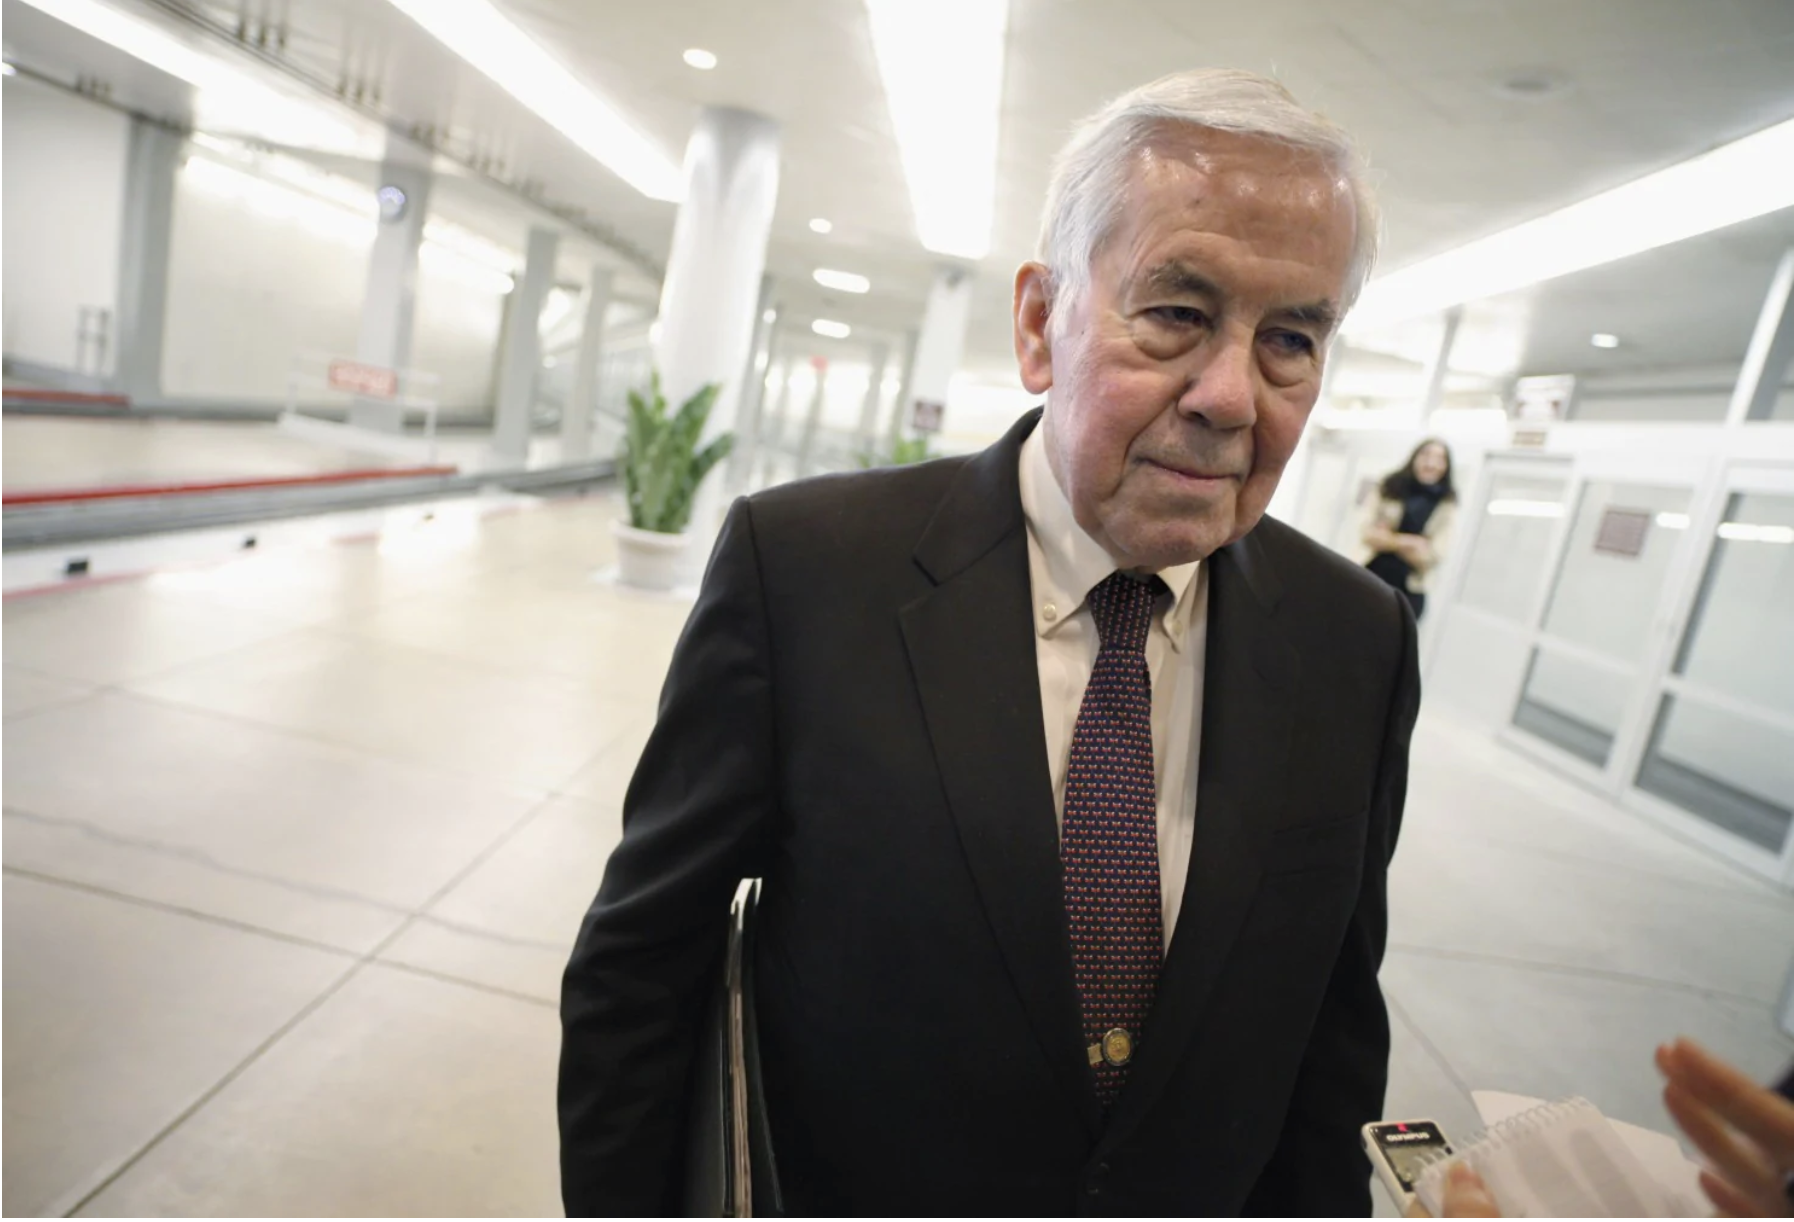
\includegraphics{../figs/DickLugar.png}}

Potomac Fever (Fenno 1978) 

\end{frame}


\begin{frame}

\Large 

\only<1>{\scalebox{0.5}{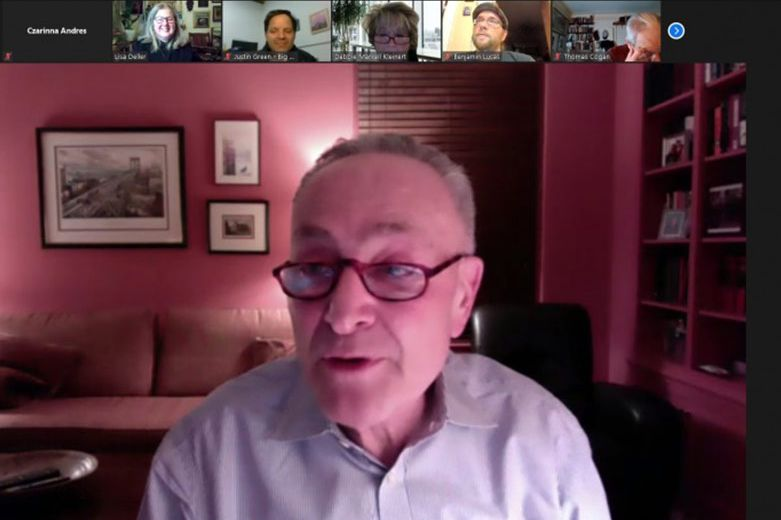
\includegraphics{../figs/SchumerNeighbor.jpeg}}} 
\only<2>{ 
\begin{center}
\scalebox{0.25}{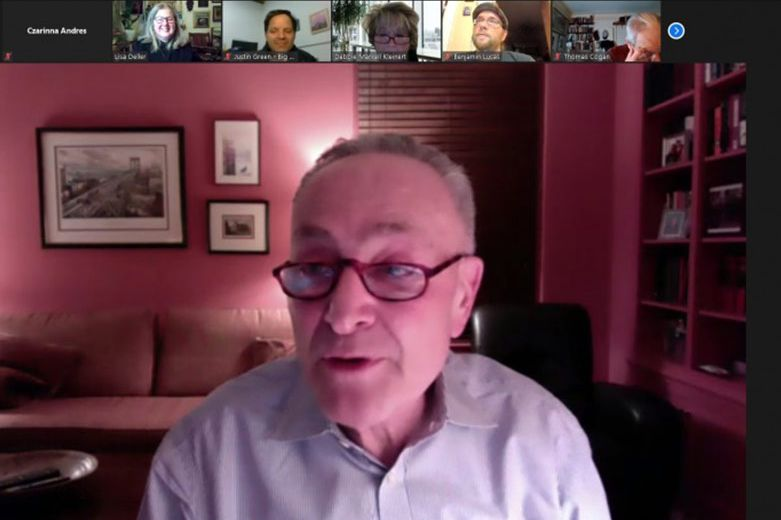
\includegraphics{../figs/SchumerNeighbor.jpeg}}
\end{center} 
\begin{itemize}
	\item Multitask accountability models: legislators acquire power, continue attention to district (\textcolor{gray}{Ashworth and Bueno de Mesquita, 2006})
	\item New legislators$\leadsto$ start-up costs 
\end{itemize}
}

\only<3>{How do legislators' attention and effort change with power and experience?\\
\bigskip
\begin{itemize}
\item[-]Shifting Priorities Hypothesis: Decrease Constituency Service?
\item[-]Increasing Capacity Hypothesis: Increase Constituency Service?
\end{itemize}
}


\end{frame}




\begin{frame}
\frametitle{Tracking Constituency Service: New Data Set}


\begin{itemize}
\item[-] Comprehensive near-census of Congressional correspondence with bureaucracy \pause 
\begin{itemize}
	\invisible<1>{\item 429 Freedom of Information Act Requests, with over 1,000 follow ups, dozens of hours on phone with FOIA officers, nearly 100 appeals of incomplete records and inappropriate denials and a small number of administrative court cases. } \pause 
	\invisible<1-2>{\item Over 487,000 Congressional correspondences} \pause 
	\invisible<1-3>{\item Builds upon important prior work that focused on specific legislator-agency pairs (\textcolor{gray}{Ritchie 2017; Mills and Kalaf-Hughes, 2015; Lowande, 2018})} \pause 
	\invisible<1-4>{\item Expansive data set enables testing theories at legislator-level} %\pause 
\end{itemize}
%\invisible<1-5>{\item  Code all Congressional Correspondence}\pause
%\begin{itemize} 
%\invisible<1-6>{\item 81\% constituency service}
%\invisible<1-6>{\item Substantial variation across legislator in number of contacts }
%\end{itemize}
\end{itemize}

\end{frame}


\begin{frame}
\frametitle{What Happens With Increased Power and Experience?}

\large 
\begin{itemize}
\item[1)] More Power\pause\invisible<1>{$\leadsto$ more correspondence. Bigger share policy focused, but not less constituency service } \pause 
\item[2)] \invisible<1-2>{More Experience}\pause\invisible<1-3>{$\leadsto$ more correspondence. Evidence of startup costs} \pause 
\end{itemize}

\invisible<1-3>{Research Design:} \pause 
\begin{itemize}
\invisible<1-4>{\item Overtime comparisons within legislator-agency pairs} \pause 
\invisible<1-5>{\item Fixed characteristics of district, legislator, and legislator's relationship with agency} \pause 
	\invisible<1-6>{\item Additional time varying controls + placebo checks  } \pause 
	\invisible<1-7>{\item Robustness checks to eliminate alternative explanations} \pause 
\end{itemize}

\invisible<1-8>{\alert{Less service$\leadsto$ New Representatives not ``Potomac Fever" } }
\end{frame}


 % \begin{frame}
 % \frametitle{Legislator Attention to the District and Constituency Service}

 % Competing expectations about how power and experience affect service:  \pause 
 %  \begin{itemize}
 %  	\invisible<1>{\item Term limit advocates/Populists: legislators attention drifts away from district and towards Washington} \pause 
 %  	\invisible<1-2>{\item Multitask + Selection models of representation: increases in legislators' budgets$\leadsto$increased constituency service   \textcolor{gray}{ (Ashworth and Bueno de Mesquita 2006)}} \pause 
 %  	\invisible<1-3>{\item Constituent demand: legislators merely respond to requests from district, little choice} \pause 
 % \end{itemize}


 % \end{frame}




\begin{frame}[label = dataslide]
\frametitle{A Near Census of Congressional Correspondence}

\only<1-3, 9->{Constituency service: ``provid[e] help to individuals, groups, and localities in coping with the federal government" (Fenno 1978)  
\begin{itemize}
	\invisible<1>{\item Identify department, agencies, and subagencies} 
	\invisible<1-2>{\item Freedom of Information Act: All contacts from members of Congress \& congressional staff 2007-2018} \pause 
	\invisible<1-8>{\item Clean, merge with Congressional data} \pause
	\invisible<1-9>{\item Hand coding \& subagency-specific inductively generated regular-expression-based coding} 	
	\pause
	\invisible<1-10>{\item Sample 10k double-coded by hand$\leadsto$ 79\% overall intercoder agreement , 90\% when coders are certain} \pause
	\invisible<1-11>{\item Contact Coding:}
		\begin{itemize}
			\invisible<1-11>{\item[-] Individual constituency service} 
			\invisible<1-11>{\item[-] Corporate constituency service}
			\invisible<1-11>{\item[-] 501c3/Local Government constituency service}
			\invisible<1-11>{\item[-] General policy }
			\invisible<1-11>{\item[-] Corporate policy } 
		\end{itemize}
\end{itemize}
\invisible<1-11>{\hyperlink{coding}{\beamerskipbutton{Definitions}}
}
}

\only<4>{\begin{scriptsize}

% Table created by stargazer v.5.2.3 by Marek Hlavac, Social Policy Institute. E-mail: marek.hlavac at gmail.com
% Date and time: Fri, Mar 29, 2024 - 15:05:16
\begin{table}[!htbp] \centering 
  \caption{Contacts From Members of Congress to Federal Agencies} 
  \label{responserates} 
\begin{tabular}{@{\extracolsep{5pt}} ccccc} 
\\[-1.8ex]\hline \\[-1.8ex] 
Department & Components FOIAed & Records received & Coded & Observations \\ 
\hline \\[-1.8ex] 
Department of Agriculture & 29 & 29 & 11 & 9603 \\ 
Department of Commerce & 19 & 18 & 10 & 7791 \\ 
Department of Defense & 49 & 13 & 7 & 9806 \\ 
Department of Education & 1 & 1 & 1 & 4676 \\ 
Department of Energy & 8 & 2 & 1 & 6256 \\ 
Department of Health and Human Services & 15 & 10 & 7 & 109701 \\ 
Department of Homeland Security & 14 & 13 & 12 & 153151 \\ 
Department of Housing and Urban Development & 2 & 1 & 1 & 32158 \\ 
Department of Justice & 23 & 6 & 3 & 3096 \\ 
Department of Labor & 22 & 12 & 9 & 62353 \\ 
Department of State & 1 & 0 & 0 & 0 \\ 
Department of Transportation & 10 & 7 & 6 & 26885 \\ 
Department of Veterans Affairs & 6 & 3 & 2 & 90808 \\ 
Department of the Interior & 11 & 8 & 6 & 6067 \\ 
Department of the Treasury & 7 & 5 & 5 & 23853 \\ 
Independent Agencies & 77 & 47 & 30 & 81152 \\ 
Total & 294 & 175 & 111 & 627356 \\ 
\hline \\[-1.8ex] 
\end{tabular} 
\end{table} 

\end{scriptsize}}

\only<5>{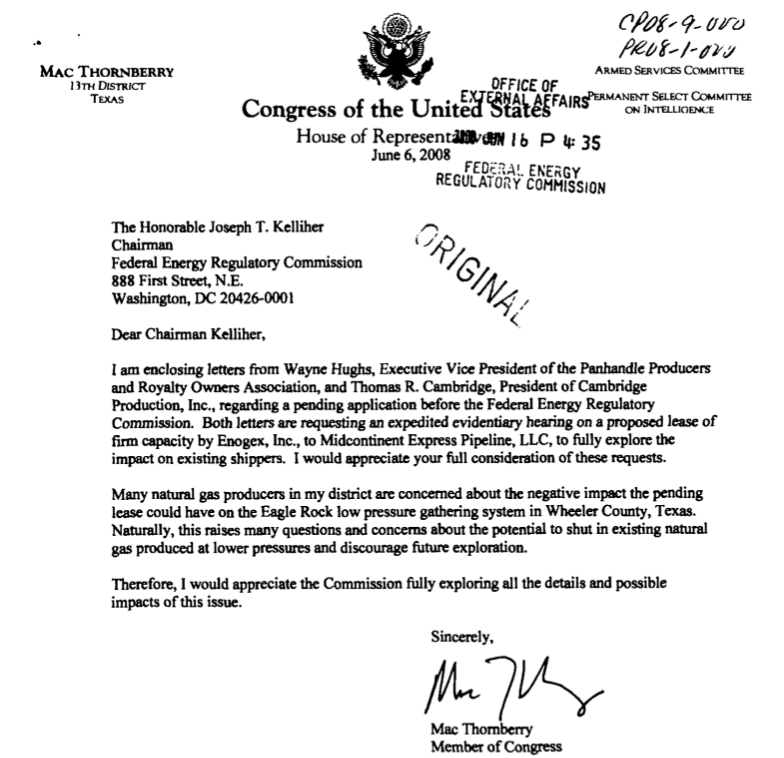
\includegraphics[width = \textwidth]{../../../correspondence/FERC.png}} 


\only<6>{Department of Homeland Security Immigration and Customs Enforcement (ICE)
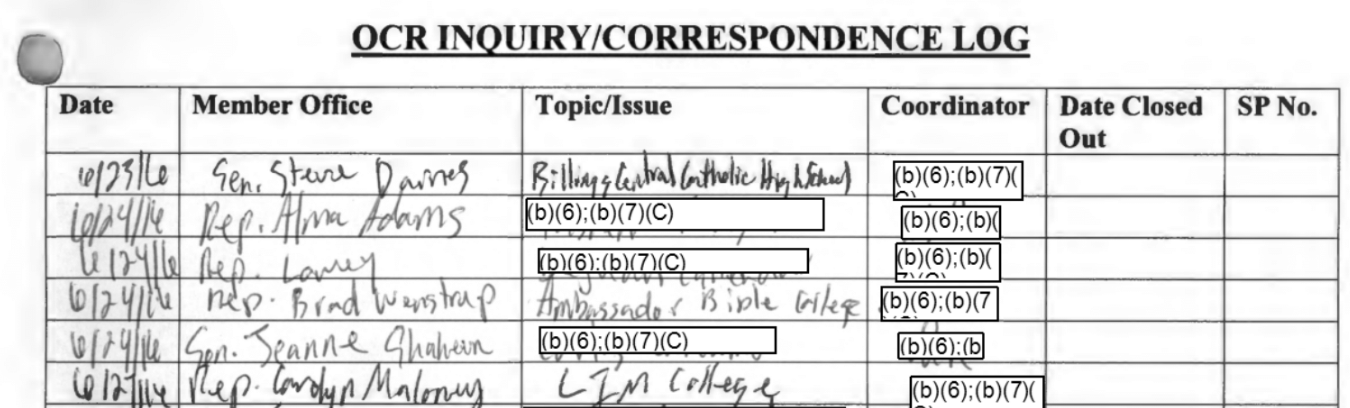
\includegraphics[width = \textwidth]{../../../correspondence/ICE.png}}


\only<7>{Environmental Protection Agency
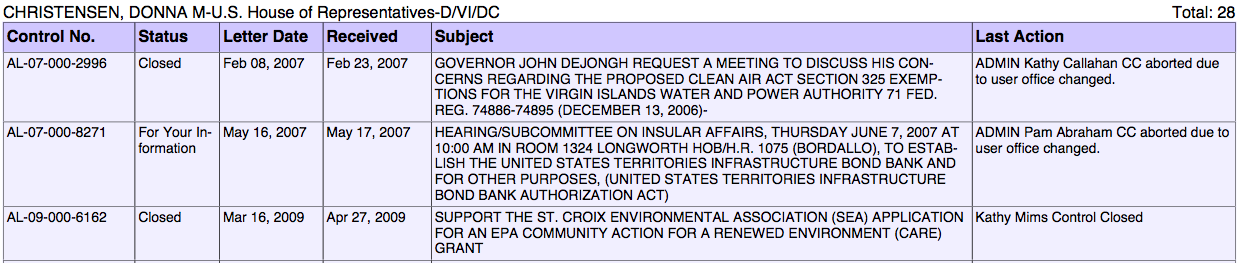
\includegraphics[width = \textwidth]{../../../correspondence/EPA.png}}

\only<8>{ Department of Homeland Security Immigration and Customs Enforcement (ICE)

\includegraphics[width = \textwidth]{../figs/schwartz.png} }




\pause \pause \pause \pause \pause \pause \pause \pause \pause 


\end{frame}


\begin{frame}
\frametitle{Who Contacts Federal Agencies?}


\only<1>{
\begin{center}
\scalebox{0.06}{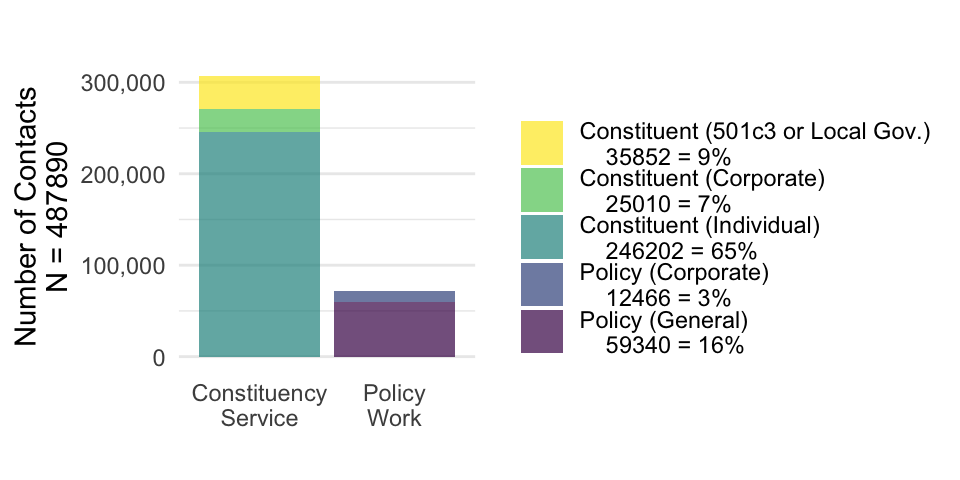
\includegraphics{figs/data_by_type-tall-1}}

\end{center}
} 


%\only<2>{\scalebox{0.3}{\includegraphics{../figs/percentiles-1}}} 

%\begin{center}
%\only<2>{\scalebox{0.5}{\includegraphics{../figs/NominateEffort.pdf}}}
%\end{center}


\end{frame}

%%%%%%%%%%%%%%%%%%%%%%%%%%
\begin{frame}
\frametitle{Highly Unequal Levels of Contact w/ Federal Agencies}
\begin{figure}
\centering

\scalebox{0.06}{\includegraphics{figs/percentiles-1}}
%\footnotetext{This figure presents the average number of contacts with federal agencies per year for House members (left-hand panel) and senators (right-hand panel), where the legislators' counts are sorted by their per year percentile rank. This reveals that senators and House members regularly contact federal agencies, but there is considerable variation in the level of contact across legislators.}
\caption{Variation in Average Legislator Requests by Percentile} \label{f:contact1} 
\end{figure}

\end{frame}
%%%%%%%%%%%%%%%%%%%%%%%%%%%%%%

\begin{frame}
\frametitle{Variation in Legislator Requests by Year 2007-2017}
\begin{figure}
\centering
%\caption{Variation in Legislator Requests by Year 2007-2017} \label{f:peryear} 
%\begin{minipage}{\textwidth}
\scalebox{0.06}{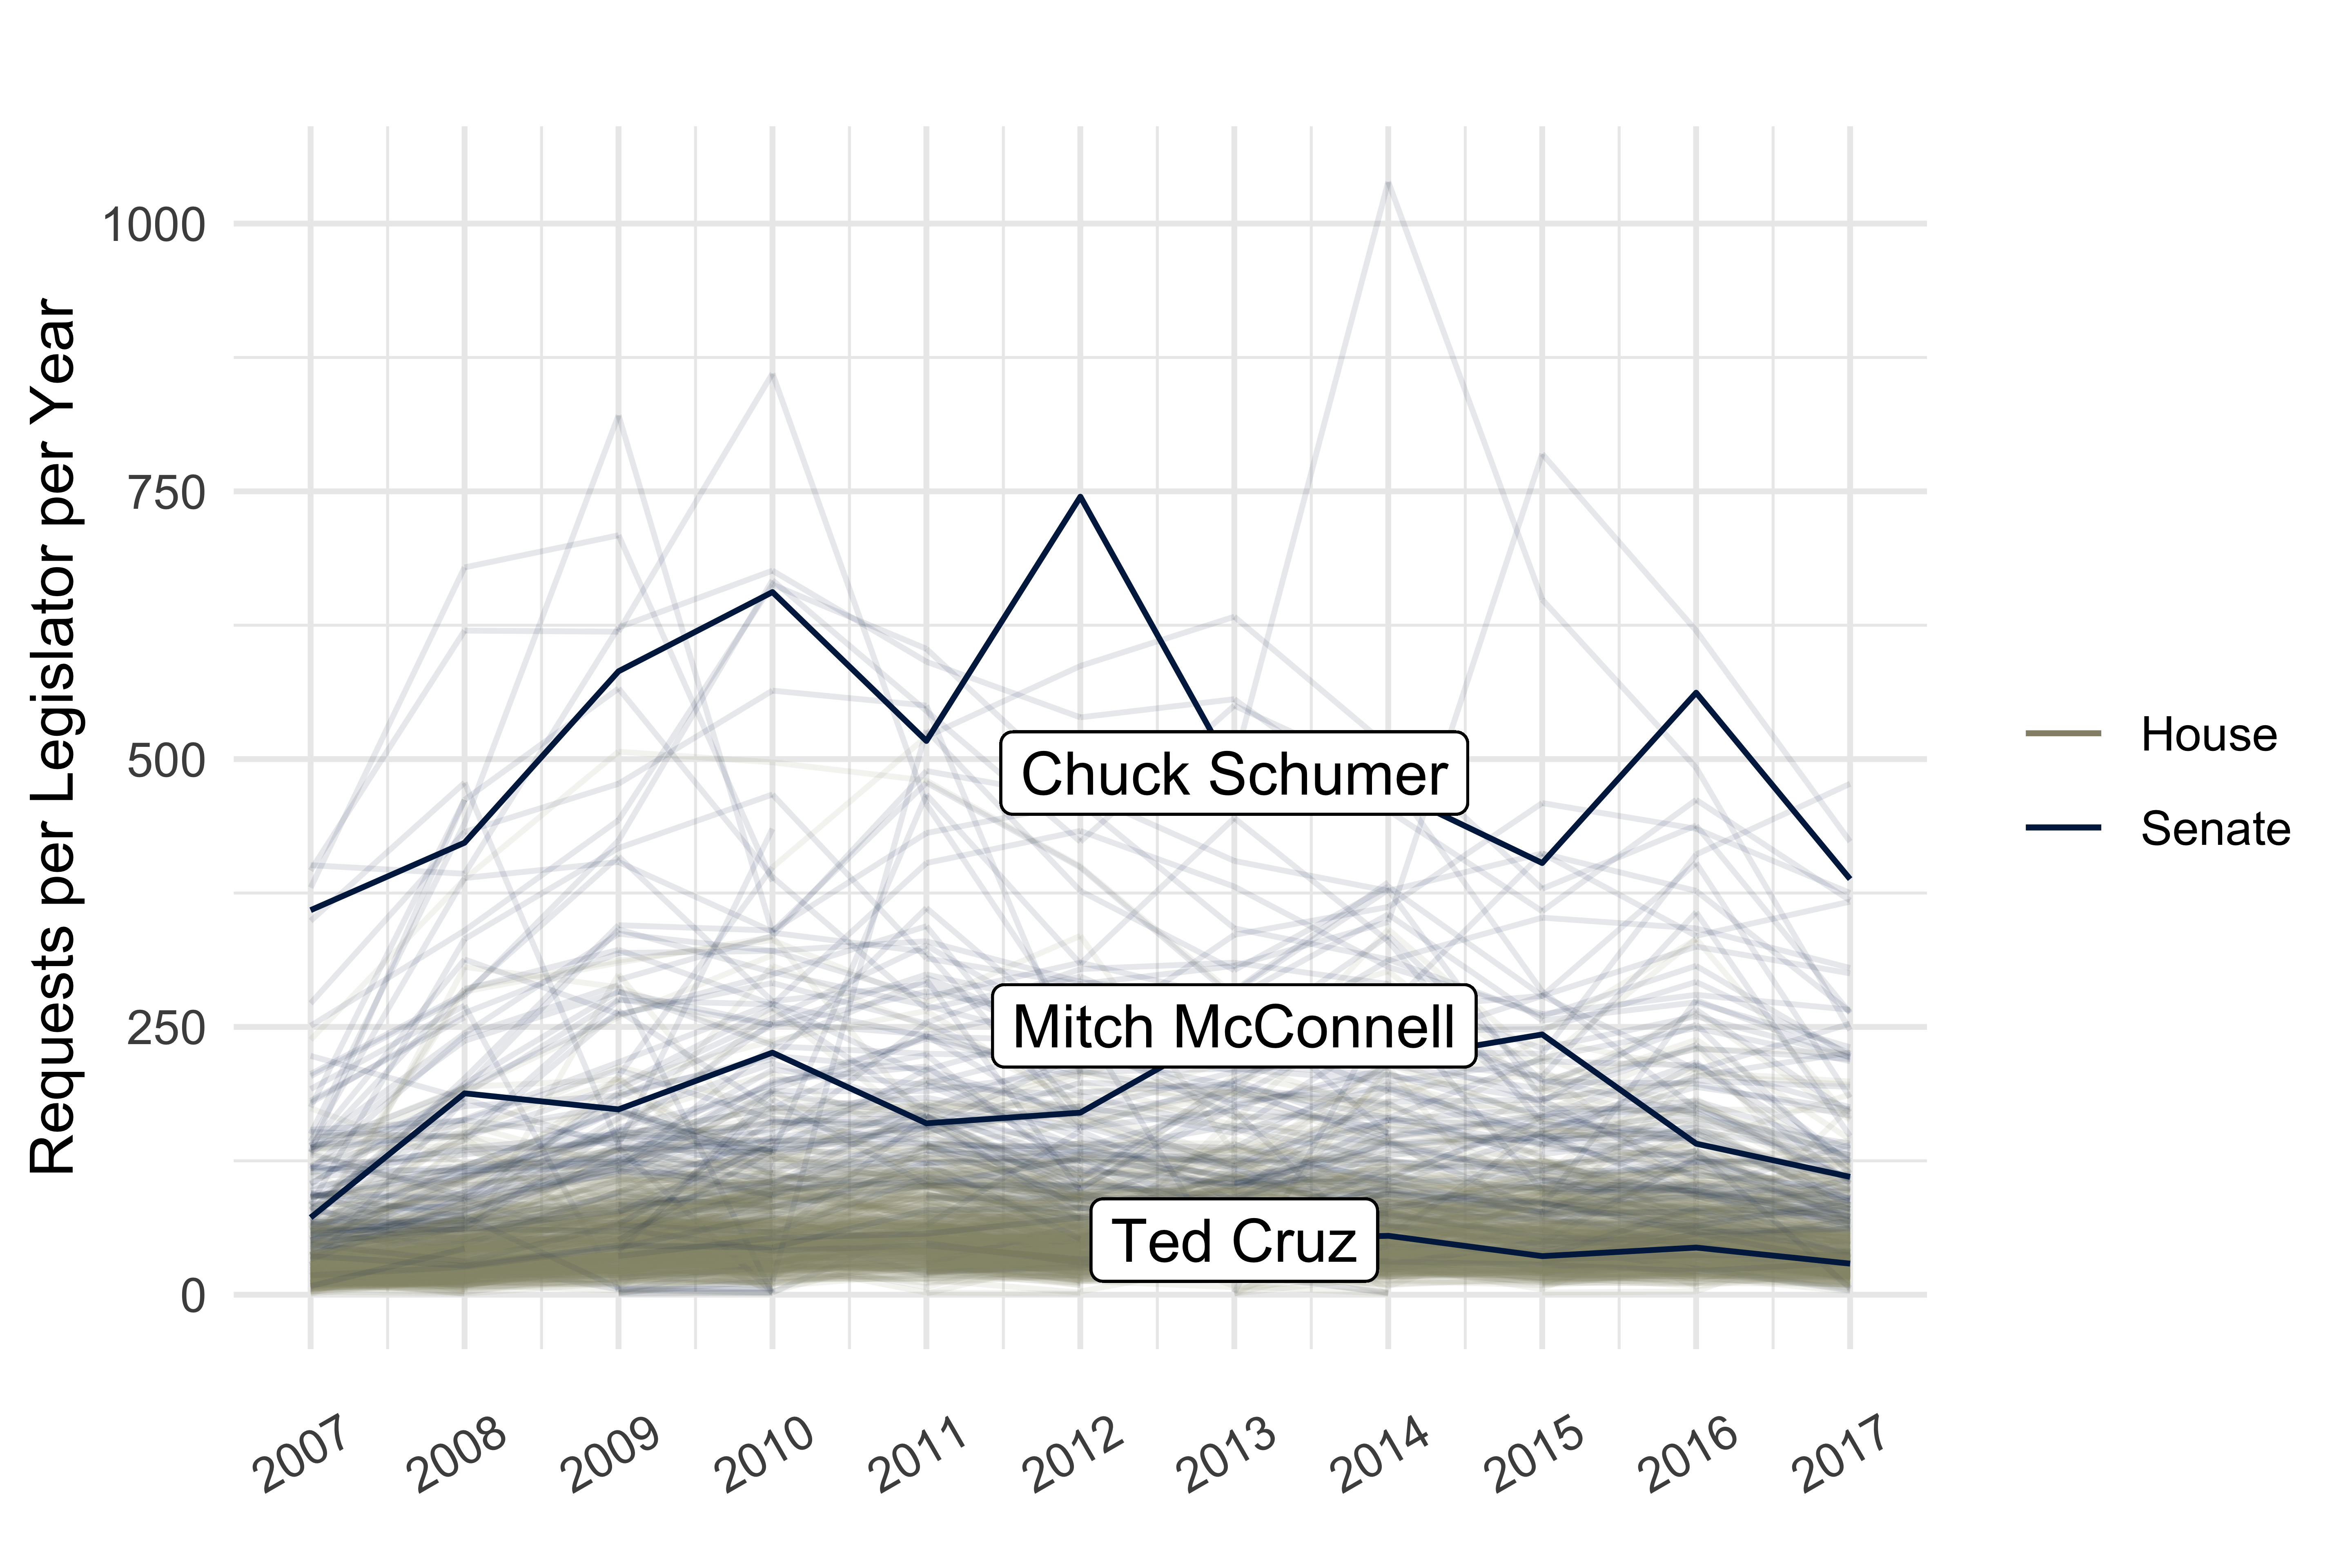
\includegraphics{figs/counts-per-year-1}}
%\footnotetext{This figure presents the number of contacts with federal agencies per year for House members (left-hand panel) and senators (right-hand panel) over time. This reveals that senators and House considerable variation in the level of contact both within and across legislators.}
%\end{minipage}
\end{figure}
\end{frame}

%%%%%%%%%%%%%%%%%%%%%%%%%%%%
\begin{frame}
\frametitle{Theory: Increasing Capacity \& Shifting Priorities}
\begin{itemize}
\item[-] \textbf{Increasing Capacity Hypothesis}: Experience \& Power Increase Constituency Service
\begin{itemize}
\item[-] Increased Resources
\item[-] Increased Organizational Efficiency
\item[-] Increased Likelihood of Success
\end{itemize}
\pause
\item[-] \textbf{Shifting Priorities Hypothesis}: Experience \& Power Decrease Constituency Service
\begin{itemize}
\item[-] As leg gain power, marginal impact of resources they allocate to policy work increases. 
\item[-] Potomac Fever: Prioritize re-election less, focus less on constituents (Fenno)
\end{itemize}
\end{itemize}

\end{frame}
%%%%%%%%%%%%%%%%%%%%%%%%%%%%%
\begin{frame}
\frametitle{Countervailing Effects of Increasing Capacity \& Shifting Priorities on Constituency Service}

\renewcommand{\arraystretch}{1.1}% THIS PADS ALL TABLES

\begin{table}[h]

%\caption{Divergent Predictions for the Change in the Levels of Constituency Service and Policy Work as Legislators Gain Experience and Power}\label{t:theory}

\begin{tabular}[t]{p{.10\linewidth}|p{.16\linewidth}|p{.27\linewidth}|p{.27\linewidth}|}

\multicolumn{2}{l}{\multirow{2}{*}{}} & \multicolumn{2}{c}{Increasing Capacity Hypothesis} \\ \cline{3-4}

\multicolumn{2}{l|}{}    &  Increase Capacity  &   No Change in Capacity \\ \cline{2-4} 

\multirow{4}{1.8cm}{Shifting Priorities Hyp.}  &   \multirow{2}{3cm}{Priority Shifts}   &  Level: 0 or $\uparrow$  &  Level of Service: $\downarrow$  \\ 

& &  Ratio of $\frac{Policy}{Service}$: $\uparrow$   &   Ratio of $\frac{Policy}{Service}$: $\uparrow$  \\ \cline{2-4}

 &  No Change    &  Level of Service: $\uparrow$  & Level of Service: $0$ \\ 

 & in Priorities &   Ratio of $\frac{Policy}{Service}$: $0$  & Ratio of $\frac{Policy}{Service}$: $0$\\ \cline{2-4}

\end{tabular}

\end{table}


\renewcommand{\arraystretch}{1}% THIS REVERTS TO NORMAL PADDING ON  ALL FUTURE  TABLES

\end{frame}
%%%%%%%%%%%%%%%%%%%%%%%%%%%
%%%%%%%%%%%%%%%%%%%%%%%%%%%%%%%%%
\begin{frame}
\frametitle{Formalizing this relationship:}

Elected Official's Policy Work: $x_i=c_i(1-p_i) $ \\
Elected Official's Constituency Service: $y_i=c_i-x_i$

\begin{itemize}
\item x: level of policy work
\item y: level of constituency service work
\item i: election official
\item c: capacity
\item $p \in [0,1]$: relative priority for constituency service versus policy work 
%\item Figure assumes a baseline capacity of 100 (e.g. 100 contacts), and a baseline ratio of constituency service to policy work of 80:20. 
\end{itemize}
\end{frame}
%%%%%%%%%%%%%%%%%%%%%%%%%%%%
\begin{frame}
\frametitle{Formalizing this relationship:}
\begin{itemize}
\item[-] When $c_{i1}p_{i1} > c_{i2}p_{i2}$, constituency service decreases. 
\item[-]When $c_{i1}p_{i1} > c_{i2}p_{i2}$, constituency service increases. 
\item[-]When $c_{i1}p_{i1} > c_{i2}p_{i2}$, constituency service stays the same.
\end{itemize}
\bigskip \pause
Key relationship: Capacity * Ratio of Constituency to Policy Work

\end{frame}
%%%%%%%%%%%%%%%%%%%%%%%%%%%%%
\begin{frame}
\frametitle{Visualizing This Relationship With A Hypothetical Example}
Figures Assume: 
\begin{itemize}
\item[-]Baseline capacity of 100 (e.g. 100 contacts)
\item[-]Baseline ratio of constituency service to policy work of 80:20. 
\end{itemize}
\end{frame}
%%%%%%%%%%%%%%%%%%%%%%%%%%%%
\begin{frame}[plain]
%\frametitle{Illustrating Countervailing Effects}
\begin{center}
\scalebox{0.4}{\includegraphics{figs/illustrateIC}}
\end{center}
\end{frame}
%%%%%%%%%%%%%%%%%%%%%%%%%%%%%
%%%%%%%%%%%%%%%%%%%%%%%%%%%%
\begin{frame}[plain]
%\frametitle{Illustrating Countervailing Effects}
\begin{center}
\scalebox{0.4}{\includegraphics{figs/illustrateSP}}
\end{center}
\end{frame}
%%%%%%%%%%%%%%%%%%%%%%%%%%%%%
%%%%%%%%%%%%%%%%%%%%%%%%%%%%
\begin{frame}[plain]
%\frametitle{Illustrating Countervailing Effects}
\begin{center}
\scalebox{0.4}{\includegraphics{figs/illustrateICSP}}
\end{center}
\end{frame}
%%%%%%%%%%%%%%%%%%%%%%%%%%%%%
%%%%%%%%%%%%%%%%%%%%%%%%%%%%
\begin{frame}[plain]
%\frametitle{Illustrating Countervailing Effects}
\begin{center}
\scalebox{0.4}{\includegraphics{figs/illustrateICSP4}}
\end{center}
\end{frame}
%%%%%%%%%%%%%%%%%%%%%%%%%%%%%
\begin{frame}
\frametitle{Alternative Explanation: Constituent Demand}
\begin{itemize}
\item[-] Differences in requests for help from constituents
\item[-] Our design limits influence of this variation: Same member representing the same district to the same agency
\begin{itemize}
\item[-] This limits extent to which differing constituent population could interfere
\end{itemize}
\end{itemize}
\end{frame}


%%%%%%%%%%%%%%%%%%%%%%%%%%%%%
\begin{frame}
\frametitle{Remaining Constituent Demand Concerns}
\begin{itemize}
\item[-] What if legislators use their official resources to encourage requests from constituents? 
\begin{itemize}
\item[-] If legislators use increased staff budget or increased organizational capacity to solicit constituent requests, demands may increase as power increases. 
\item[-] Consistent with our theory \& may be key mechanism
\item[-] Not an exogenous shift in constituent demand that could confound our analysis
\end{itemize}
\pause
\item[-] What if constituents direct requests toward powerful legislators?
\begin{itemize}
\item[-] Robustness checks
\item[-] No evidence of requests spilling over to more experienced members in delegation
\end{itemize}
\end{itemize}
\end{frame}
%%%%%%%%%%%%%%%%%%%%%%%%%%%%%
\begin{frame}[label = SpecReturn]
\frametitle{Assessing the Effect of Committee Power and Experience}

Goal: estimate effect of increased power and experience in Congress on number of contacts per agency \pause 

\begin{itemize}
	\invisible<1>{\item Cross-sectional comparison} \pause 
	\begin{itemize}
		\invisible<1-2>{\item[-] Descriptive differences are important} \pause
		\invisible<1-3>{\item[-] Conflates ability with position } \pause
		\invisible<1-4>{\item[-] Difficult to identify a set of covariates to disentangle} \pause
	\end{itemize}
	\invisible<1-5>{\item Panel Design} \pause 
	\begin{itemize}
		\invisible<1-6>{\item[-] Difference-in-differences at the legislator-agency level} \pause 
		\invisible<1-7>{\item[-] Examine within legislator-agency change} \pause 
		\invisible<1-8>{\item[-] Include time-varying characteristics (majority party, president's party)} \pause 
		\invisible<1-9>{\item[-] Cluster standard errors at the legislator-level}
	\end{itemize}		
\end{itemize}

\hyperlink{spec}{\beamerskipbutton{Specification}}

\end{frame}
%%%%%%%%%%%%%%%%%%%%%%%%%%%%%%%%%%%%%%%%%
\begin{frame}

\begin{figure}[hbt!]
\centering
\caption{The Effect of Experience and Institutional Power on Constituency Service: (Within Legislator Diff-in-Diff) } \label{f:m-total-predicted}
\scalebox{0.1}{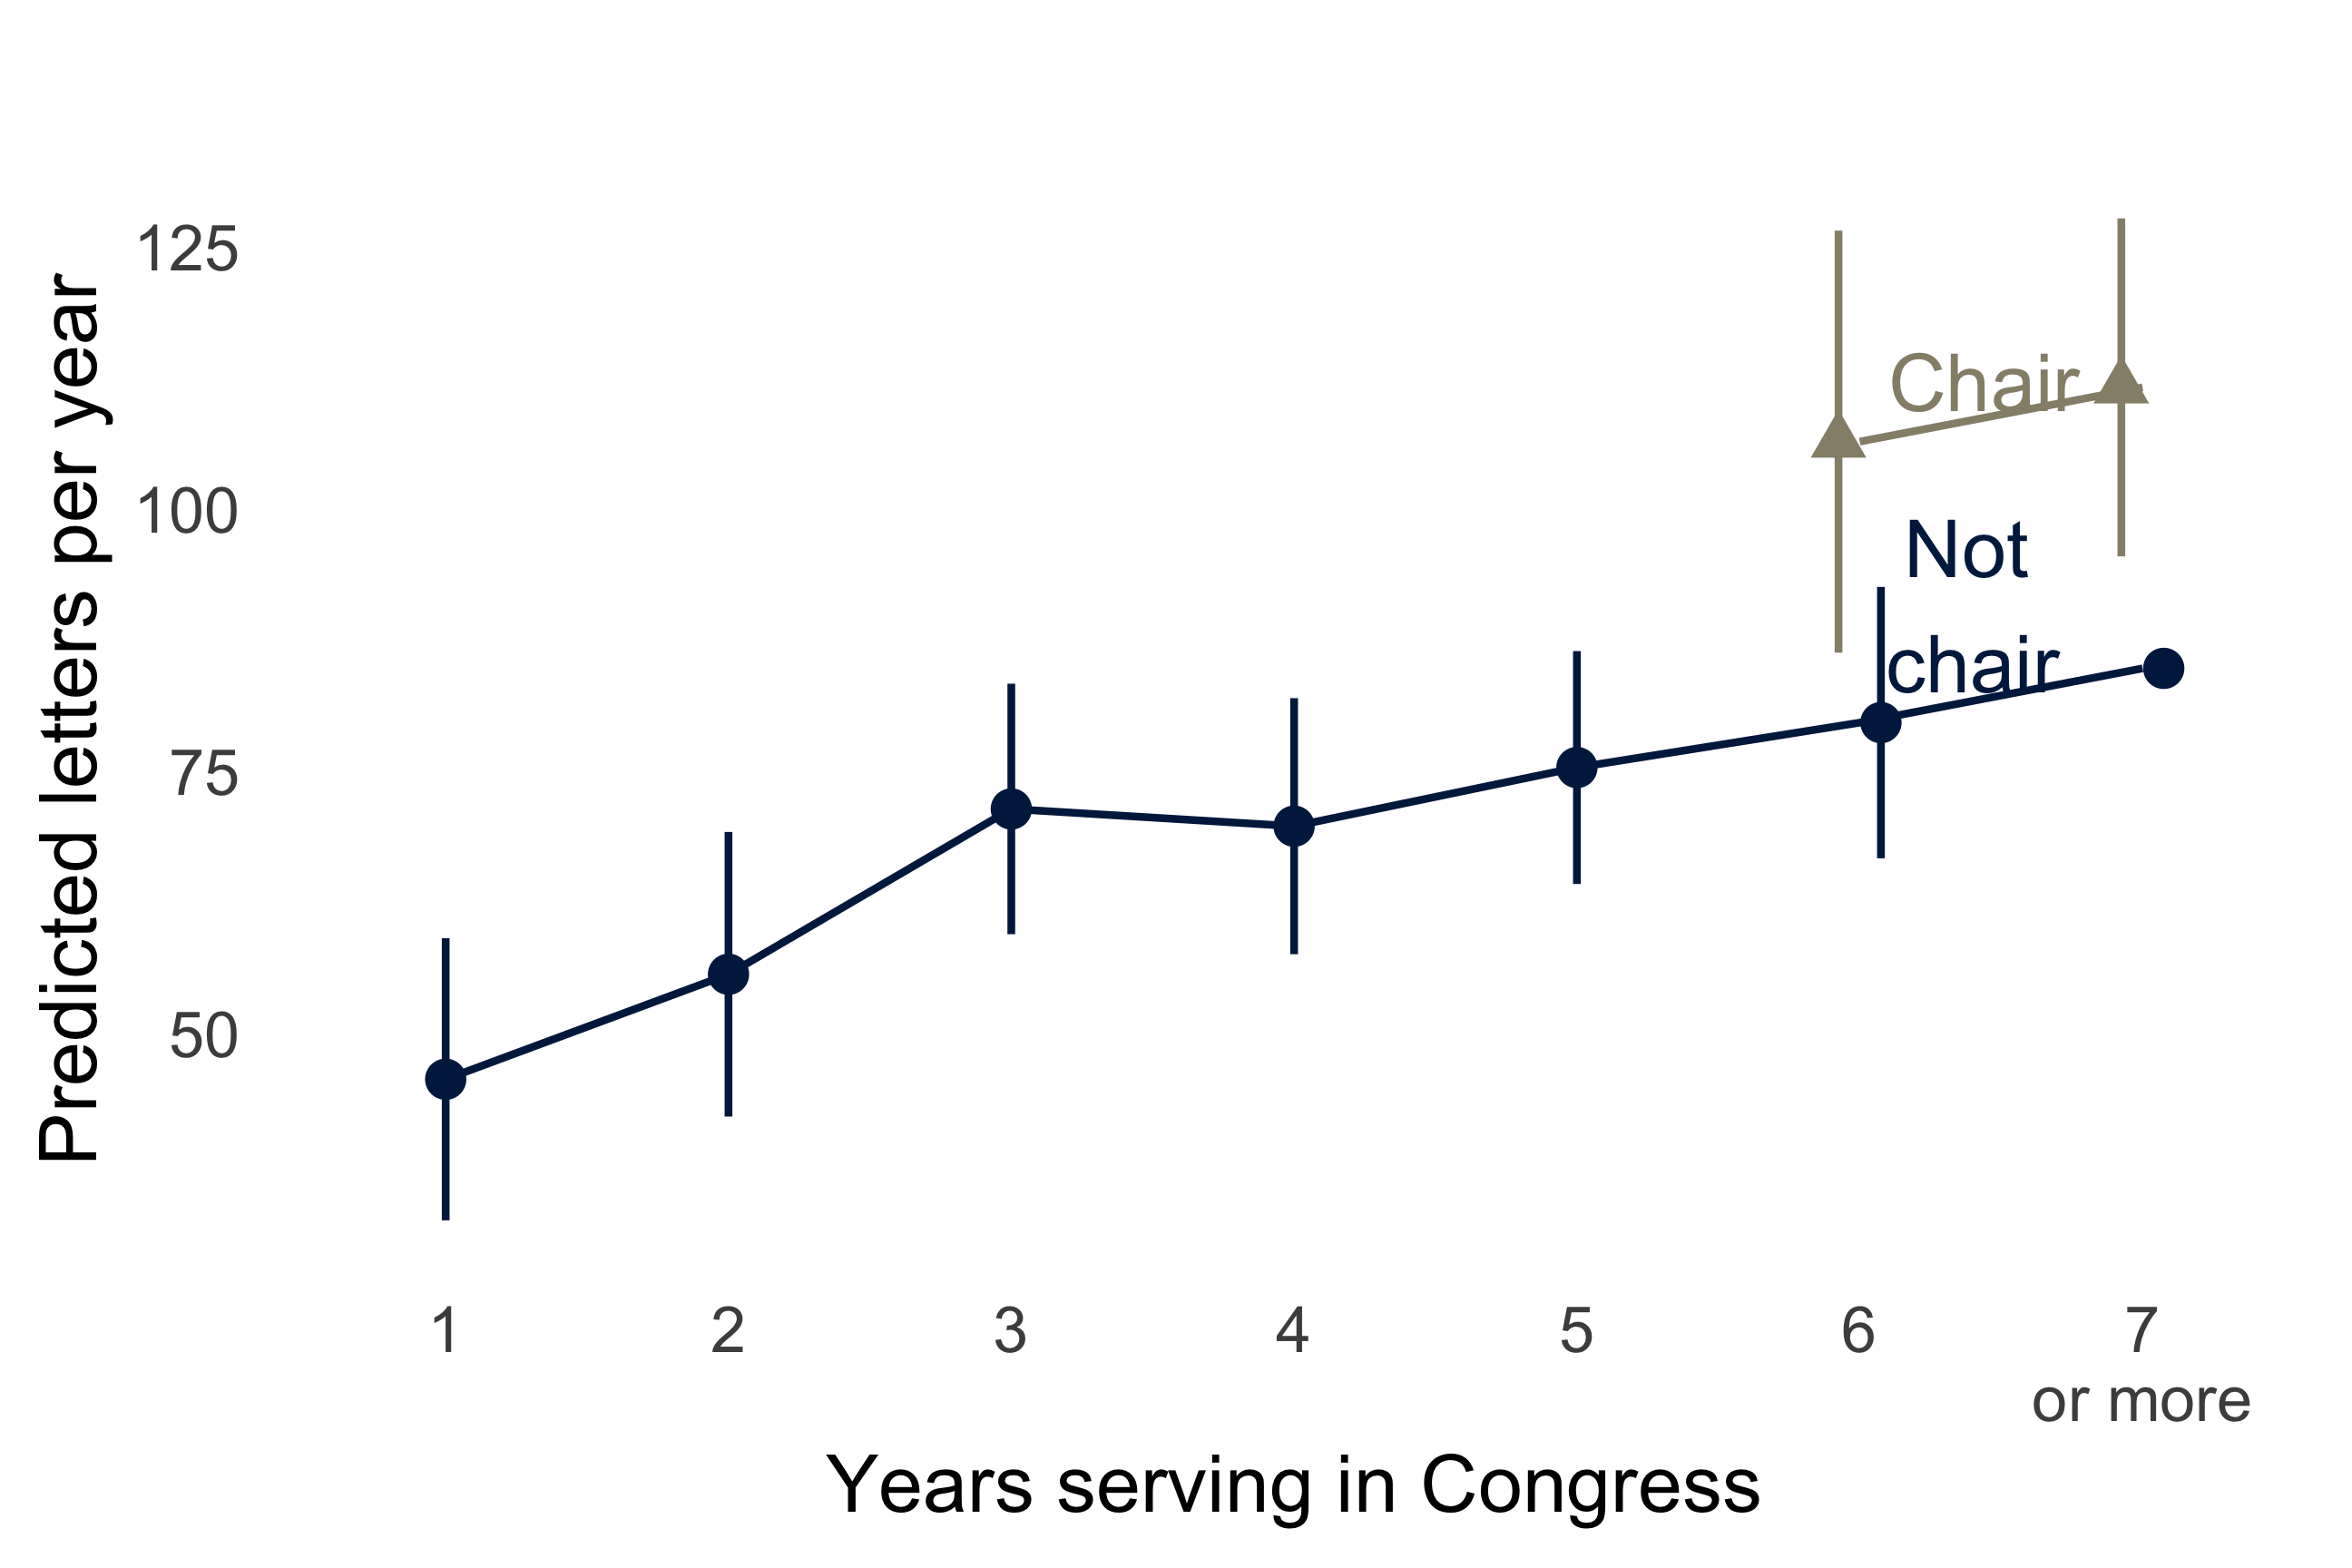
\includegraphics{figs/m-total-predicted-4}}
\end{figure}
\end{frame}
%%%%%%%%%%%%%%%%%%%%%%%%%%%%%%%%%
\begin{frame}
\frametitle{Effect of Increased Resources and Prestige}

\begin{itemize}
	\item $\approx$ 24 additional contacts per year when becoming chair, smaller effects for ranking member or prestige committee 
	\end{itemize}
\end{frame}
%%%%%%%%%%%%%%%%%%%%%%%%%%%%%%%%%%%

\begin{frame}[label= tenure]

\frametitle{Start Up Costs and New Legislators}
\begin{itemize}
\item Within legislator analysis: early career legislator, less service (compared to later in career) \pause 
\begin{itemize}
\item New legislator districts have 35 fewer service requests.
\item Takes about 6 years to learn.
\end{itemize}
\invisible<1>{\item Within district analysis: replace legislator, less service (compared to previous incumbent)} \pause 
\end{itemize}

\invisible<1-2>{\alert{Rather than experienced legislators turning from district, new legislators are less equipped to deliver service}}


\hyperlink{district}{\beamerskipbutton{Within District}}
\end{frame}

%%%%%%%%%%%%%%%%%%%%%%%%%%%%
\begin{frame}
\frametitle{Shifting Priorities?}
Dependent Variable: $\frac{\# of policy requests}{\# of constituency service requests}$ per legislator per year

\end{frame}
%%%%%%%%%%%%%%%%%%%%%%%%%%%%%%%%
\begin{frame}
%\frametitle{The Effect of Experience \& Institutional Power on Legislators' Priorities}

\scalebox{.1}{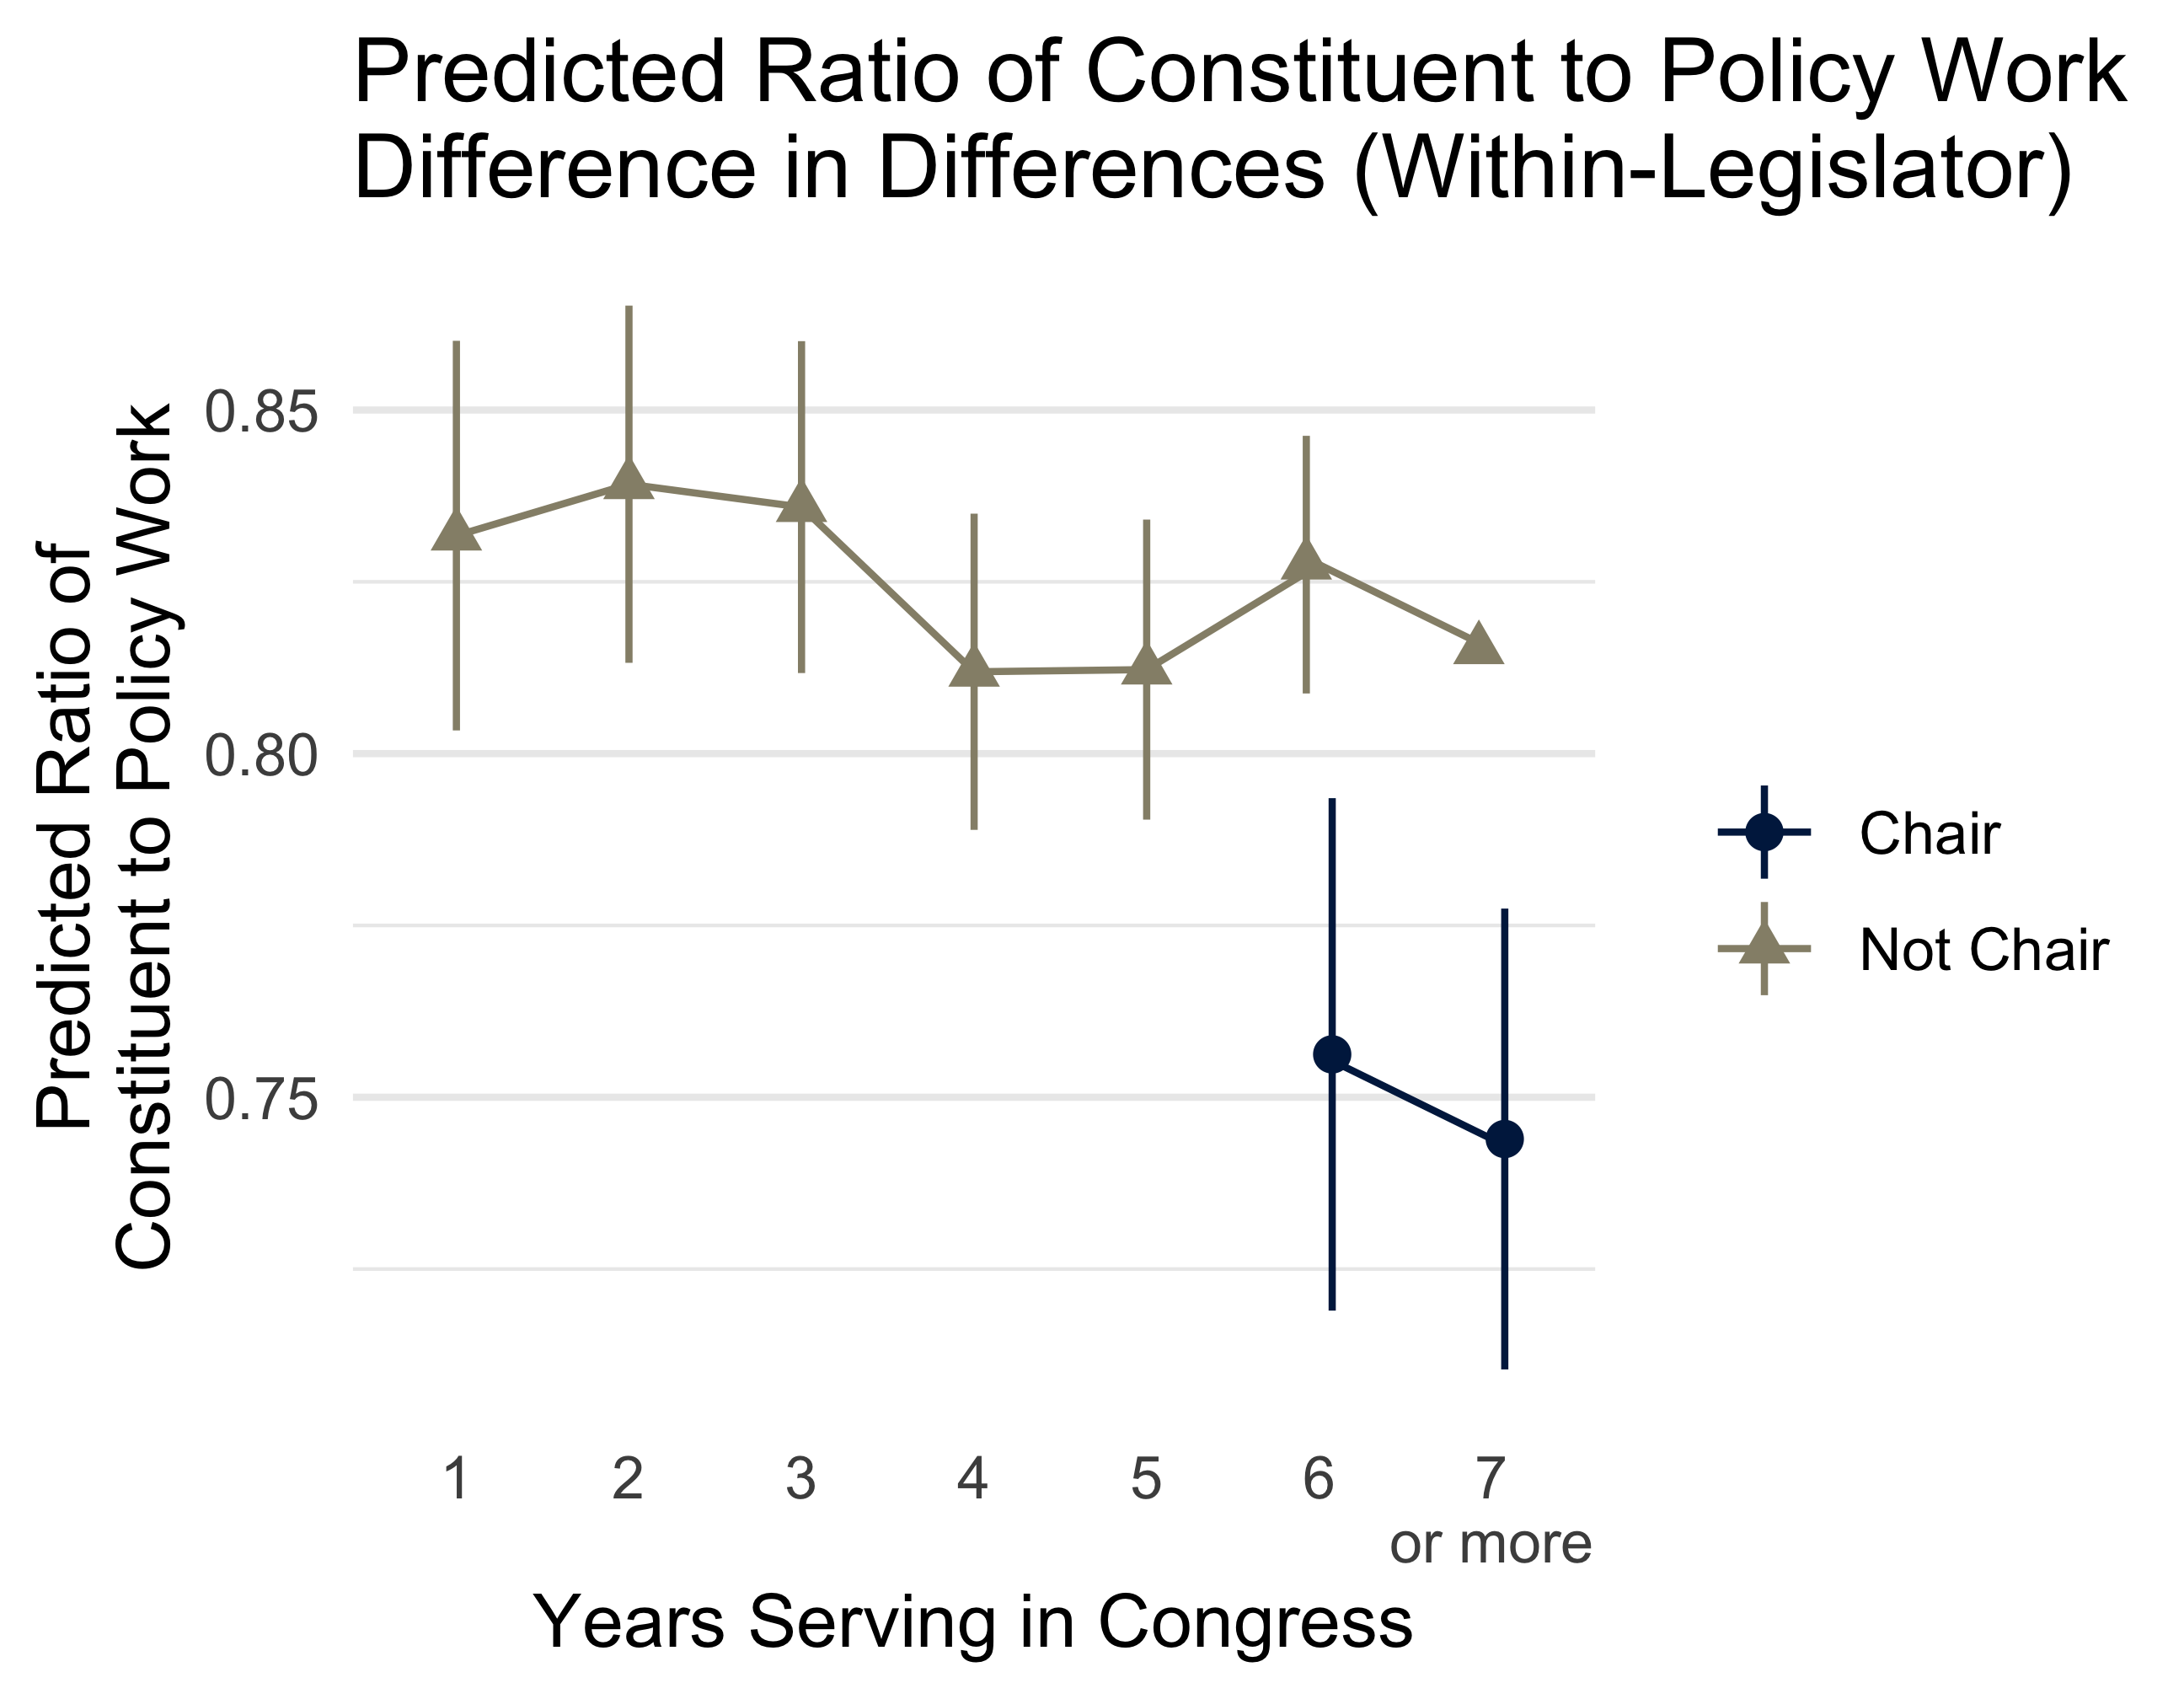
\includegraphics{figs/m-ratio-predicted-4}}



\end{frame}
%%%%%%%%%%%%%%%%%%%%%%%%%%%%%%
%\begin{frame}
%\frametitle{Is This Just Constituent Demand?}

%Are legislators merely reacting to constituent demand? %\pause 
%\begin{itemize}
%	\invisible<1>{\item Research design addresses static and slow-moving demand} \pause 
%%	\invisible<1-2>{\item Demand for constituency service can (and often is) created$\leadsto$ different mechanism} \pause 
%	\invisible<1-3>{\item But do constituents direct requests to more powerful and experienced legislators?} %\pause 
%\end{itemize}


%Examine implications of this objection
%\begin{itemize}
%	\item[1)] Name recognition decreases slowly over legislators' career
%	\item[2)] Little evidence constituents redirect requests
%\end{itemize}	



%\end{frame}
%%%%%%%%%%%%%%%%%%%%%%%
\begin{frame}
\frametitle{The Effects of Demand for Constituency Service}
\begin{itemize}
\item[-]District Characteristics Affect the Provision of Constituency Service
\begin{itemize}
\item[-] State Population for Senate
\item[-] Veteran Population in District for VA contact
\item[-] Population Over 65 for Social Security Admin contact
\end{itemize}
\end{itemize}
\end{frame}
%%%%%%%%%%%%%%%%%%%%%%%%
%%%%%%%%%%%%%%%%%%%%%%%%%%%%%%
\begin{frame}
\frametitle{Is This Just Constituent Demand?}

Are legislators merely reacting to constituent demand? \pause 
\begin{itemize}
	\invisible<1>{\item Research design addresses static and slow-moving demand} \pause 
	\invisible<1-2>{\item Demand for constituency service can (and often is) created$\leadsto$  mechanism} \pause 
	\invisible<1-3>{\item But do constituents direct requests to more powerful and experienced legislators?} \pause 
\end{itemize}


Examine implications of this objection
\begin{itemize}
\item[-] Examined Spillover from New Legislators
\begin{itemize}
\item[-] The proportion of a state delegation that is new
\item[-] Indicator for new member in delegation
\end{itemize}
\item[-] Little evidence constituents redirect requests

\end{itemize}	



\end{frame}


\begin{frame}
\frametitle{Conclusion}


\alert{Experienced and powerful legislators deliver service to the district} \pause 

\begin{itemize}
 \invisible<1>{\item Evidence in favor of both Increasing Capacity and Shifting Priorities}\pause
  \invisible<1-2>{\item Increase in Capacity Outweighs Shift in Priorities}\pause
	\invisible<1-3>{\item No tradeoff for Constituents: As legislators acquire power, also ``deliver the goods" to district} \pause 
	\invisible<1-4>{\item \alert{Start up Costs} of electing new legislators } \pause 
\invisible<1-5>{\item Implications for Theory: Scholars should focus on both level of effort and how they divide that effort} \pause 
\invisible<1-6>{\item Implications for Policy: 
\begin{itemize}
\item[-] Congressional Staffing
\item[-] Term Limits}
\end{itemize}
\pause 
\end{itemize}
\bigskip
\invisible<1-7>{Ongoing research$\leadsto$ representation, campaign finance, and congressional connection with agencies} 



\end{frame}


\appendix

\begin{frame}

\begin{center}
Thank you!

{\tt eleanor.powell@wisc.edu}
%{\tt jgrimmer@stanford.edu}

\end{center}


\end{frame}



\begin{frame}[label = spec]
\frametitle{Estimating Effect of Increasing Committee Prestige on Contacts}

\begin{eqnarray}
Y_{ijt} & = & \beta \text{Committee Position}_{it}   + \gamma_{ij} +  \delta_{tj} + \sum_{s = 1}^{S} \eta_{s} \text{tenure}_{s[it]} + m_{it} + p_{it} +  \epsilon_{ijt}  \nonumber 
\end{eqnarray}

Where: \pause 
\begin{itemize}
	\invisible<1>{\item  $Y_{ijt} = $ Number of contacts between legislator $i$ and agency $j$ in year $t$} \pause 
	\invisible<1-2>{\item $\beta = $ Estimated causal effect of obtaining committee position } 
		\begin{itemize}
		\invisible<1-2>{	\item[1)] Chair of committee}
		\invisible<1-2>{	\item[2)] Ranking member }
		\invisible<1-2>{	\item[3)] Prestige committee assignment}
		\invisible<1-2>{	\item[4)] Oversight committee assignment}\pause 
		\end{itemize}
	\invisible<1-3>{\item  $\gamma_{ij} = $ Legislator $i$ x Agency $j$ fixed effect }
	\invisible<1-3>{\item  $\delta_{tj} = $ Year $t$ x Agency $j$ fixed effect}\pause
	\invisible<1-4>{\item $m_{it}, p_{it},\sum_{s = 1}^{S} \eta_{s} \text{tenure}_{s[it]} $ time varying controls } \pause 
\end{itemize}

\invisible<1-5>{Standard errors clustered at legislator level} %(same results if clustered at legislator level)}

\hyperlink{SpecReturn}{\beamerskipbutton{Return}}

\end{frame}


\begin{frame}
\frametitle{Institutional Research}

\begin{tiny} 
\textbf{Legislators' expressed agenda and credit claiming }

\begin{itemize}
	\item[-] Books: Grimmer (2013), Grimmer, Westwood, and Messing (2014)
	\item[-] Articles: Grimmer (2010), Grimmer and King (2011), Grimmer, Messing, and Westwood (2012), Grimmer (2013), Grimmer (2015)
\end{itemize}

\textbf{The value of Congressional Committees (and Congressional Careers)}
\begin{itemize}
	\item[-] Articles: Grimmer and Powell (2013), Powell and Grimmer (2016) 
\end{itemize}


\textbf{Gender Composition and Discussion Dynamics}
\begin{itemize}
	\item[-] Article: Ban, Grimmer, Kaslovsky, and West (2022)
\end{itemize}

\textbf{Constituency Service and Congressional Careers}
\begin{itemize}
	\item[-] Book: Grimmer, Judge-Lord, and Powell (Congressional Representation: Constituents, Donors, and Policy)
	\item[-] Articles: Judge-Lord, Grimmer, and Powell (2022), Powell, Judge-Lord, and Grimmer (2022) 
	\item[-] Future work: polarization and service, lettermarking, and embedding to describe legislator engagement with agencies.
\end{itemize}

\textbf{Social Media and Legislative Communication}
\begin{itemize}
	\item[-] Articles: Grimmer, Lim, and Lee (2016), Grimmer and Lee (2017)
\end{itemize} 

\textbf{Presidency and Executive} 
\begin{itemize}
	\item[-] Articles: Carpenter and Grimmer (2009), Carpenter, Grimmer, and Lomazoff (2011), Franco, Grimmer, and Lim (2016) 
\end{itemize}

\textbf{Election Administration}
\begin{itemize}
\item[-] Articles: Grimmer, Hersh, Meredith, and Nall (2018), Grimmer and Yoder (2021), Eggers, Garro, and Grimmer (2021) 	
\end{itemize}


\textbf{Related Methods Work:}
\begin{itemize}
	\item[-] Articles: Fong and Grimmer (2016), Grimmer, Messing, and Westwood (2017), Fong and Grimmer (2022), Grimmer, King, Superti, and Tyler (2022), Grimmer, Feinstein, Hersh, and Carpenter (2011)  
\end{itemize} 	

\end{tiny}

\end{frame}



\begin{frame}[label = coding]
\frametitle{Category Definitions}


\only<1>{1 = Personal Service\\

\hfill\begin{minipage}{\dimexpr\textwidth-2cm}
Definition: Individual, non-commercial constituent service. \\
Examples: Help with a government form, passport, visa, back pay, military honor, enlistment, criminal case, request for personal information (e.g., one's FBI file), disability application, worker compensation, personal complaint, discrimination case, job application, health insurance, financial services complaints, etc. \\
\end{minipage}
}

\only<2>{2 = Commercial Service - Transactional \\

\hfill\begin{minipage}{\dimexpr\textwidth-2cm}
Definition: Anything related to a specific individual case by a business (including business owners like farmers and consultants).\\ 
General Examples: Help with a grant application, payment, loan, or contract (buying anything from or selling anything to a government agency). Help with an individual case of tax assessment, fine, or regulatory enforcement action. Help with public relations on behalf of a business.\\
Specific Examples: allocation of radio spectrum, a case against a company, tax dispute, contract for the purchase of military surplus, crop insurance distribution, debt settlement, foreclosure assistance, a fine for a law violation, etc. \\
\end{minipage} } 

\only<3>{3 = Government and Nonprofit Service - Transactional\\

\hfill\begin{minipage}{\dimexpr\textwidth-2cm}
Definition: Same as for (2-Commercial Service), but for municipal or state governments (including cities, counties, etc.) or non-business-oriented nonprofit organizations (i.e., NOT ones that represent an industry or trade association) \\
\end{minipage} } 

\only<4>{4 = Commercial Service - Policy \\

\hfill\begin{minipage}{\dimexpr\textwidth-2cm}
Definition: Anything applying to a class of commercial activity or businesses (e.g., shipping, airlines, agriculture), including legislation, bills, acts, appropriations, authorizations, etc. \\
General Examples: Authorization of or appropriation to a government program targeted towards a particular industry or industries. Regulation of industry or commercial practice or competition.\\
Specific Examples: Milk prices, insurance or loan eligibility criteria, purchasing policies, crop insurance rates, pollution criteria, classification of products for trade or taxation, conservation appropriation, worker visa types, restrictions, or caps, etc.\\
\end{minipage} } 
 
\only<5>{5 = Policy Work - NOT in the service of any individual, business, specific industry.\\

\hfill\begin{minipage}{\dimexpr\textwidth-2cm}
Examples of Policy Work: 
 \begin{itemize} 
 \item Lawmaking 
\item Request for policy-relevant information. This includes prospective legislation, legislation under consideration, or already implemented legislation that requires oversight.  
\item Oversight
\item Committee requesting a report or testimony at a hearing
\item Requesting clarity on an agency rule
\item Lobbying administrative policy
\item Agency rulemaking with non-commercial implications (comments on agency rulemaking may often be (3)) 
\item Political work
\item Meeting with organized constituent groups (e.g. workers, people with disabilities, environmentalists) about policy (meetings with industry groups generally fall under (4)).
\item Media requests
 \end{itemize} 
\end{minipage}
\bigskip } 


\only<6>{6 = Other \\

\hfill\begin{minipage}{\dimexpr\textwidth-2cm}
	Suggest a new category in the NOTES column, only if you cannot fit it under 1-4. For example, requesting dirt on one's political opponents could be called ``partisan" as none of the above. Other specific types: thank you (for thank you notes with no other information), congratulations (for congratulatory correspondence on appointments or retirements with no other information), family member (for correspondence on behalf of a family member) \\
\end{minipage}} 
\pause \pause \pause \pause \pause 



\hyperlink{dataslide}{\beamerskipbutton{Return}}



\end{frame}



\begin{frame}[label=district]


\begin{footnotesize}
\begin{tabular}{l*{4}{c}}
\toprule
                    &\multicolumn{1}{c}{(1)}&\multicolumn{1}{c}{(2)}&\multicolumn{1}{c}{(3)}&\multicolumn{1}{c}{(4)}\\
\midrule
New Legislator      &      -35.23&      -35.55&      -14.89&      -123.5\\
                    &     (4.445)&     (4.500)&     (2.627)&     (13.84)\\
Legislator 2nd Year &      -23.75&      -20.31&      -4.402&      -79.99\\
                    &     (4.464)&     (3.949)&     (2.662)&     (11.34)\\
Legislator 3rd Year &      -13.08&      -13.53&      -1.630&      -49.48\\
                    &     (4.886)&     (4.448)&     (2.586)&     (16.07)\\
Legislator 4th Year &      -12.43&      -9.077&       0.268&      -26.92\\
                    &     (5.216)&     (4.276)&     (2.736)&     (16.30)\\
Legislator 5th Year &      -14.92&      -11.58&      -3.810&      -31.58\\
                    &     (4.416)&     (3.591)&     (2.128)&     (13.11)\\
Legislator 6th Year &      -13.56&      -5.216&      -1.638&      -2.500\\
                    &     (5.104)&     (3.790)&     (2.239)&     (14.46)\\
\midrule
District Fixed Effects&            &  \checkmark&  \checkmark&  \checkmark\\
Year Fixed Effects  &            &  \checkmark&  \checkmark&  \checkmark\\
All Districts       &  \checkmark&  \checkmark&            &            \\
House Only          &            &            &  \checkmark&            \\
Senate Only         &            &            &            &  \checkmark\\
Observations        &        6578&        6578&        5338&        1240\\
\bottomrule
\multicolumn{5}{l}{\footnotesize Robust standard errors in parentheses, clustered at district level}\\
\end{tabular}

\end{footnotesize}

\hyperlink{tenure}{\beamerskipbutton{Tenure Slide}}

\end{frame}



\begin{frame}[label=party]
\frametitle{What are Legislators Contacting Federal Agencies About?}
\scalebox{0.5}{\includegraphics{../figs/NominateEffort.pdf}}
\end{frame}

\begin{frame}
\frametitle{Descriptive Evidence about Power and Experience}
\begin{center}
\only<2>{	
\begin{table}[ht]
\centering
\begin{tabular}{l|cc}
  \hline
  Rank & Contacts per Agency & \% Constituency Service\\ 
  \hline
 Members & 0.99 & 82\% \\ 
 Ranking Minority & 1.87 & 79\% \\ 
 Chair & 1.86 & 74\% \\ 
   \hline
\end{tabular}
\caption{Average Number of Contacts by Institutional Position}
\end{table}
}

\end{center} 


\begin{center}
\only<3>{
	\scalebox{0.45}{\includegraphics{../figs/TenureDifference.pdf}}
}
\end{center}



\end{frame}
%%%%%%%%%%%%%%%%%%%%%%%
\begin{frame}
\frametitle{Example: The Effect of Electing New Legislators in Wisconsin}

\only<1>{\scalebox{0.06}{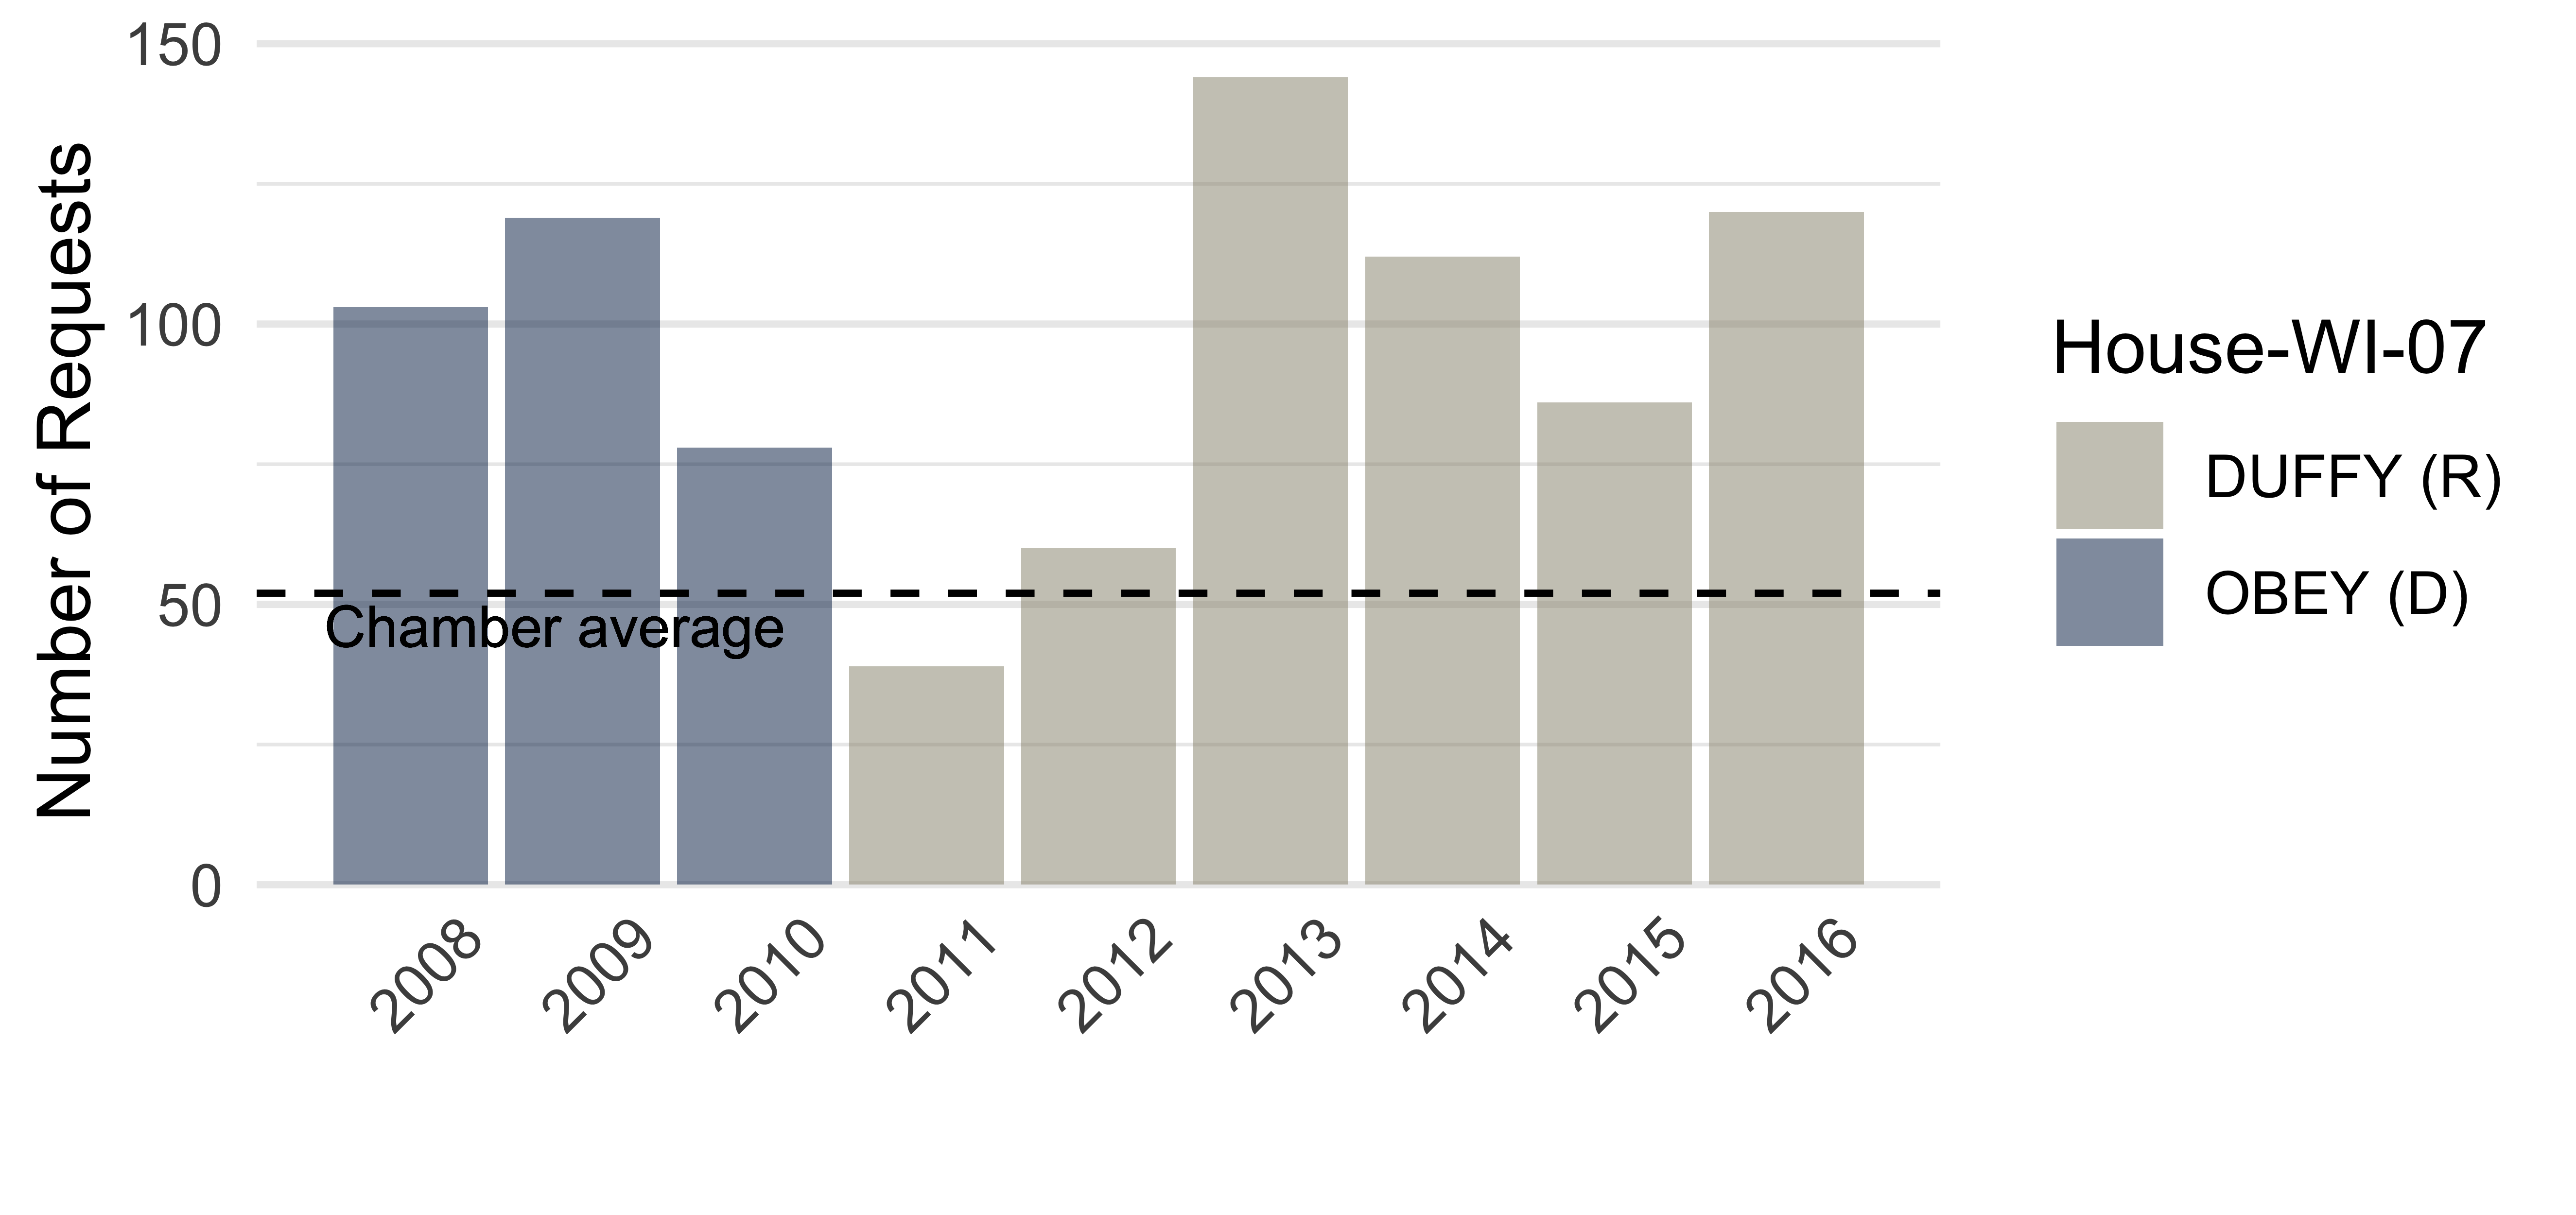
\includegraphics{figs/districts/(WI-07)}}}
\only<2>{\scalebox{0.06}{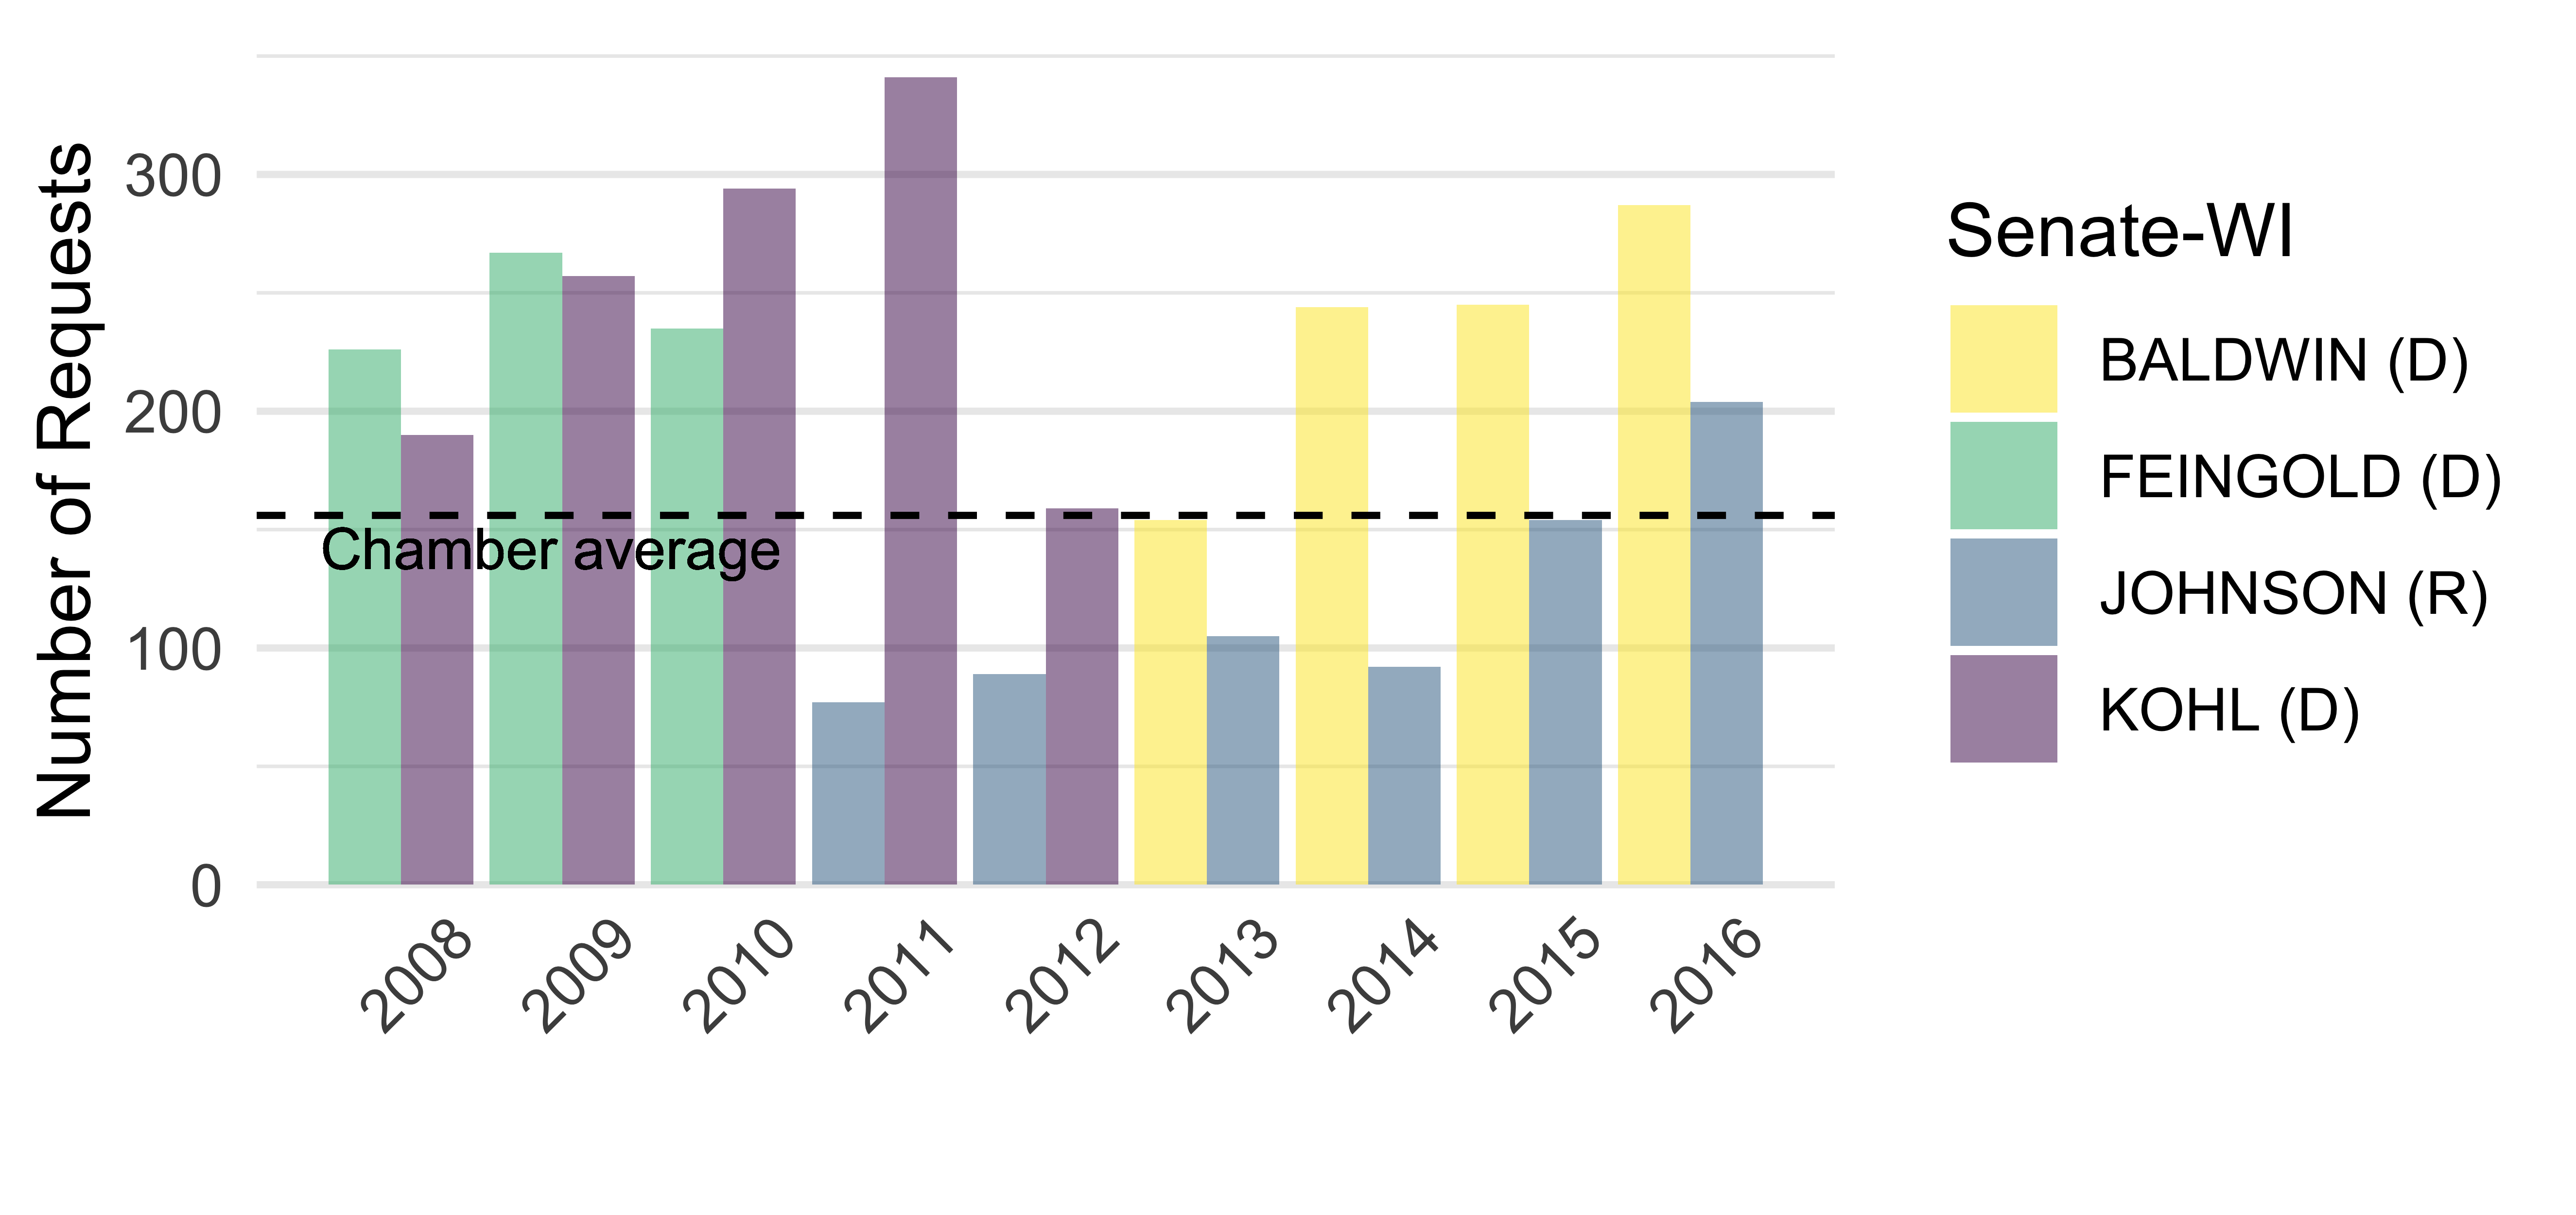
\includegraphics{figs/districts/(WI)}}}
\end{frame}







%\frametitle{Correspondence Data}
% For example, here Rep. Thornberry, chair of armed services committee is writing to Federal Energy Regulatory Commission on behalf of two companies in his district, asking for extra scrutiny on a another company's permit application. 

% We have several thousand such letters written to this agency, which we use optical content recognition to extract the text. If they do not have metadata like the sender's name and date, we extract it from the text of the letter or discription of the letter.

%\frametitle{Correspondence Data}




%\frametitle{Correspondence Data}

% rich and informative summaries like those kept by the EPA. Here, Rep Donna writes about a regulatory exemption for a power plant, to alert EPA to a hearing, and in support of a nonprofit grant application.

%\begin{frame}
%\frametitle{New Facts About Legislator Contact with Federal Agencies}

%\only<1>{\scalebox{0.5}{\includegraphics{../figs/TypeHistogram1.pdf}}}

%\only<2>{\scalebox{0.5}{\includegraphics{../figs/TypeHistogram2.pdf}}}

%\only<3>{\scalebox{0.3}{\includegraphics{/users/justingrimmer/correspondence/Figs/percentiles-1}}}

%\only<4>{\scalebox{0.3}{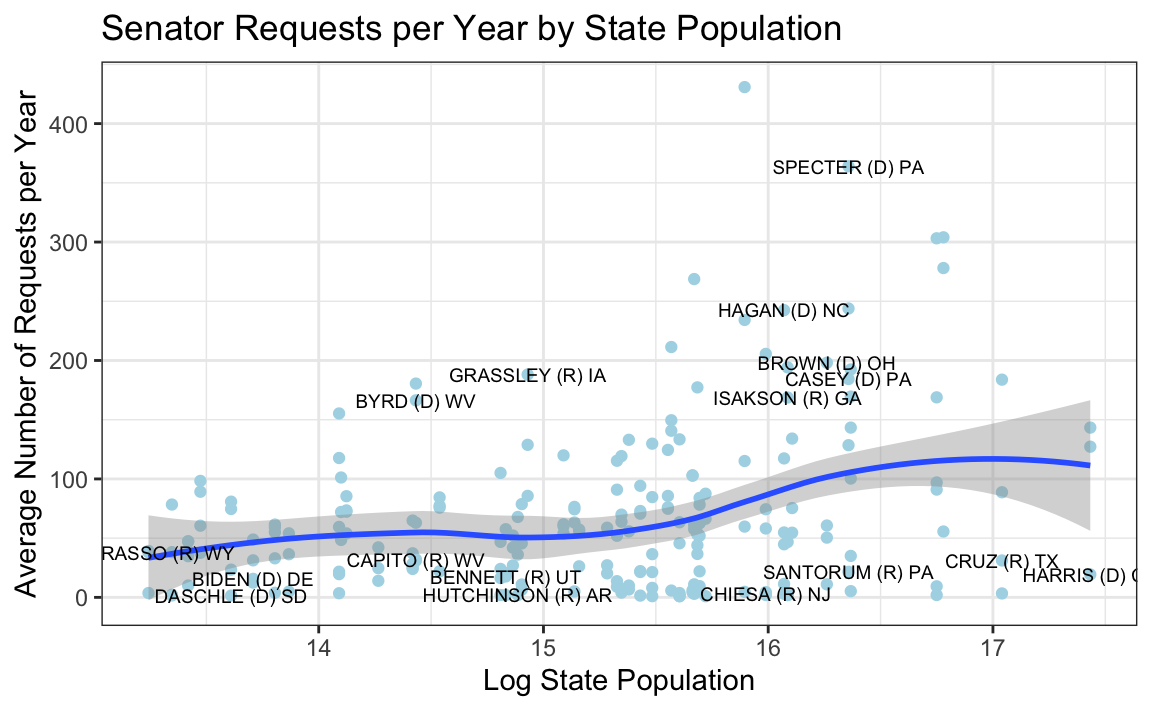
\includegraphics{/users/justingrimmer/correspondence/Figs/population-1}}}

%\only<5>{
%	District demographics are correlated with types of requests legislators make
%	\begin{itemize}
%		\item Higher proportion of veterans $\leadsto$ more requests to VA
%		\item Higher proportion of residents over 65 $\leadsto$ more requests to SSA 
%	\end{itemize}		
%}

%\end{frame}



\end{document}